% Options for packages loaded elsewhere
\PassOptionsToPackage{unicode}{hyperref}
\PassOptionsToPackage{hyphens}{url}
\documentclass[
  ignorenonframetext,
  aspectratio=169,
]{beamer}
\newif\ifbibliography
\usepackage{pgfpages}
\setbeamertemplate{caption}[numbered]
\setbeamertemplate{caption label separator}{: }
\setbeamercolor{caption name}{fg=normal text.fg}
\beamertemplatenavigationsymbolsempty
% remove section numbering
\setbeamertemplate{part page}{
  \centering
  \begin{beamercolorbox}[sep=16pt,center]{part title}
    \usebeamerfont{part title}\insertpart\par
  \end{beamercolorbox}
}
\setbeamertemplate{section page}{
  \centering
  \begin{beamercolorbox}[sep=12pt,center]{section title}
    \usebeamerfont{section title}\insertsection\par
  \end{beamercolorbox}
}
\setbeamertemplate{subsection page}{
  \centering
  \begin{beamercolorbox}[sep=8pt,center]{subsection title}
    \usebeamerfont{subsection title}\insertsubsection\par
  \end{beamercolorbox}
}
% Prevent slide breaks in the middle of a paragraph
\widowpenalties 1 10000
\raggedbottom
\AtBeginPart{
  \frame{\partpage}
}
\AtBeginSection{
  \ifbibliography
  \else
    \frame{\sectionpage}
  \fi
}
\AtBeginSubsection{
  \frame{\subsectionpage}
}
\usepackage{iftex}
\ifPDFTeX
  \usepackage[T1]{fontenc}
  \usepackage[utf8]{inputenc}
  \usepackage{textcomp} % provide euro and other symbols
\else % if luatex or xetex
  \usepackage{unicode-math} % this also loads fontspec
  \defaultfontfeatures{Scale=MatchLowercase}
  \defaultfontfeatures[\rmfamily]{Ligatures=TeX,Scale=1}
\fi
\usepackage{lmodern}
\ifPDFTeX\else
  % xetex/luatex font selection
\fi
% Use upquote if available, for straight quotes in verbatim environments
\IfFileExists{upquote.sty}{\usepackage{upquote}}{}
\IfFileExists{microtype.sty}{% use microtype if available
  \usepackage[]{microtype}
  \UseMicrotypeSet[protrusion]{basicmath} % disable protrusion for tt fonts
}{}
\makeatletter
\@ifundefined{KOMAClassName}{% if non-KOMA class
  \IfFileExists{parskip.sty}{%
    \usepackage{parskip}
  }{% else
    \setlength{\parindent}{0pt}
    \setlength{\parskip}{6pt plus 2pt minus 1pt}}
}{% if KOMA class
  \KOMAoptions{parskip=half}}
\makeatother
\usepackage{longtable,booktabs,array}
\usepackage{caption}
\captionsetup[table]{skip=6pt}
\newcounter{none} % for unnumbered tables
\usepackage{calc} % for calculating minipage widths
\usepackage{caption}
% Make caption package work with longtable
\makeatletter
\def\fnum@table{\tablename~\thetable}
\makeatother
\usepackage{graphicx}
\makeatletter
\newsavebox\pandoc@box
\newcommand*\pandocbounded[1]{% scales image to fit in text height/width
  \sbox\pandoc@box{#1}%
  \Gscale@div\@tempa{\textheight}{\dimexpr\ht\pandoc@box+\dp\pandoc@box\relax}%
  \Gscale@div\@tempb{\linewidth}{\wd\pandoc@box}%
  \ifdim\@tempb\p@<\@tempa\p@\let\@tempa\@tempb\fi% select the smaller of both
  \ifdim\@tempa\p@<\p@\scalebox{\@tempa}{\usebox\pandoc@box}%
  \else\usebox{\pandoc@box}%
  \fi%
}
% Set default figure placement to htbp
\def\fps@figure{htbp}
\makeatother
\setlength{\emergencystretch}{3em} % prevent overfull lines
\providecommand{\tightlist}{%
  \setlength{\itemsep}{0pt}\setlength{\parskip}{0pt}}
% Auto-generated by infrastructure/rendering/_pdf_latex_helpers.py::extract_math_font_preamble.
% Minimal header passed to Pandoc via -H so Beamer slides pick up the same math font
% as the combined-PDF path. Adjust the manuscript's preamble.md to change the font globally.
\usepackage{unicode-math}
\setmathfont{latinmodern-math.otf}

% Manuscript macro/package fallbacks (newcommand -> providecommand).
% Core mathematics
\usepackage{amsmath}
\usepackage{amssymb}
% Document layout
% Tables
\usepackage{booktabs}
% Caption styling (booktabs already loaded above). Small caption font with a
% bold label ("Figure 1", "Table 2") gives the math/figure-heavy layout a
% consistent, journal-like caption rhythm without fighting pandoc-crossref —
% pandoc emits standard \caption{}, and caption/captionsetup only restyle it.
% ── Theorem environments ─────────────────────────────────────────────────
% amsthm is loaded above. The FedGVI<->Friston bridge is stated as a small
% number of theorems/definitions/lemmas/propositions/corollaries; sharing one
% counter (definition/lemma/proposition/corollary all step the `theorem`
% counter) gives a single monotone numbering 1, 2, 3, ... across all kinds, so
% authors can reference them as Theorem 1, Definition 2, Corollary 3 without a
% per-kind counter drifting out of order. Plain style for theorem-like results,
% definition style (upright body) for definitions.
% (algorithm2e intentionally not loaded: this manuscript states results as
% numbered amsthm Theorems/Definitions, not algorithm2e pseudocode.)
% Code listings
\usepackage{listings}
% Typography and formatting
% (siunitx intentionally not loaded: no \SI/\num units appear in this manuscript.)
% Cross-references and citations
% (cleveref and titlesec intentionally not loaded: unavailable in this TeX tree
% and not required. Cross-references resolve through pandoc-crossref's own
% \ref-style names — no \cref appears — and section heading styling falls back
% to the pandoc/LaTeX defaults.)
% ── TeX Live Basic-compatible mono font for code listings ────────────
% Latin Modern Mono is bundled with TeX Live Basic and keeps the manuscript
% renderable on minimal TeX installations. Mathematical Unicode coverage is
% provided separately by Latin Modern Math below, so the code font does not
% need a private JuliaMono installation.
%
% Use the TeX font filename rather than the system-family name: the minimal
% TeX Live fontconfig database may not register the OpenType family even though
% kpsewhich can resolve the bundled files.
% Math font for unicode-math: Latin Modern Math (TeX Live) has full BMP
% coverage including U+2223 (\mid), U+226A/226B (\ll/\gg), and the Greek/
% blackboard letters used in equations. Without an explicit \setmathfont,
% unicode-math falls back to lmroman text font which lacks several glyphs
% and emits "Missing character" warnings on every \mid in math mode.

% Slide layout defaults for warning-clean scientific decks.
\usepackage{etoolbox}
\IfFileExists{xurl.sty}{\usepackage{xurl}}{}
\IfFileExists{seqsplit.sty}{\usepackage{seqsplit}}{\newcommand{\seqsplit}[1]{#1}}
\protected\def\breakseq#1{\seqsplit{#1}}
\protected\def\breaktt#1{\begingroup\ttfamily\seqsplit{#1}\endgroup}
\setlength{\emergencystretch}{6em}
\tolerance=5000
\hbadness=10000
\hfuzz=1pt
\setlength{\tabcolsep}{2pt}
\AtBeginEnvironment{longtable}{\tiny\renewcommand{\arraystretch}{0.86}\setlength{\tabcolsep}{1pt}}
\AtBeginEnvironment{tabular}{\tiny\renewcommand{\arraystretch}{0.86}\setlength{\tabcolsep}{1pt}}
\AtBeginEnvironment{equation}{\tiny}
\AtBeginEnvironment{equation*}{\tiny}
\AtBeginEnvironment{align}{\tiny}
\AtBeginEnvironment{align*}{\tiny}
\AtBeginEnvironment{itemize}{\footnotesize}
\AtBeginEnvironment{enumerate}{\footnotesize}
\AtBeginEnvironment{description}{\footnotesize}
\setbeamerfont{caption}{size=\tiny}
\setbeamerfont{caption name}{size=\tiny}
\setbeamerfont{normal text}{size=\small}
\setbeamerfont{frametitle}{size=\small}
\setbeamerfont{section title}{size=\footnotesize}
\setbeamerfont{subsection title}{size=\footnotesize}
\setbeamertemplate{section page}{%
  \centering
  \begin{beamercolorbox}[sep=12pt,center,wd=\paperwidth]{section title}
    \parbox{0.86\paperwidth}{\centering\usebeamerfont{section title}\insertsection\par}
  \end{beamercolorbox}
}
\setbeamertemplate{subsection page}{%
  \centering
  \begin{beamercolorbox}[sep=8pt,center,wd=\paperwidth]{subsection title}
    \parbox{0.86\paperwidth}{\centering\usebeamerfont{subsection title}\insertsubsection\par}
  \end{beamercolorbox}
}
\setlength{\abovecaptionskip}{2pt}
\setlength{\belowcaptionskip}{0pt}

% Natbib and cross-reference fallbacks — slides don't load natbib
% or cleveref, but combined-PDF manuscript prose may emit these
% commands. The fallback renders citations as a bracketed key list
% and cross-references as detokenized labels so slides don't fail on
% undefined control sequences or raw underscores. \providecommand is
% a no-op if packages load later.
\providecommand{\citep}[1]{[#1]}
\providecommand{\citet}[1]{#1}
\providecommand{\citealp}[1]{#1}
\providecommand{\citeauthor}[1]{#1}
\providecommand{\citeyear}[1]{#1}
\providecommand{\cref}[1]{\texttt{\detokenize{#1}}}
\providecommand{\Cref}[1]{\texttt{\detokenize{#1}}}
\providecommand{\crefrange}[2]{\texttt{\detokenize{#1}}--\texttt{\detokenize{#2}}}
\providecommand{\Crefrange}[2]{\texttt{\detokenize{#1}}--\texttt{\detokenize{#2}}}
\providecommand{\paragraph}[1]{\textbf{#1}\ }

% Opt-in accessible presentation profile.
\setbeamerfont{normal text}{size*={20pt}{24pt}}
\setbeamerfont{frametitle}{size*={28pt}{32pt}}
\setbeamerfont{section title}{size*={28pt}{32pt}}
\setbeamerfont{subsection title}{size*={28pt}{32pt}}
\setbeamerfont{caption}{size*={16pt}{19pt}}
\setbeamerfont{caption name}{size*={16pt}{19pt}}
\setbeamerfont{itemize/enumerate body}{size*={20pt}{24pt}}
\setbeamerfont{itemize/enumerate subbody}{size*={20pt}{24pt}}
\setbeamerfont{itemize/enumerate subsubbody}{size*={20pt}{24pt}}
\setbeamerfont{itemize item}{size*={20pt}{24pt}}
\setbeamerfont{itemize subitem}{size*={20pt}{24pt}}
\setbeamerfont{itemize subsubitem}{size*={20pt}{24pt}}
\setbeamerfont{description body}{size*={20pt}{24pt}}
\setbeamerfont{description item}{size*={20pt}{24pt}}
\setbeamerfont{quote}{size*={20pt}{24pt}}
\setbeamerfont{quotation}{size*={20pt}{24pt}}
\AtBeginEnvironment{longtable}{\fontsize{20pt}{24pt}\selectfont}
\AtBeginEnvironment{tabular}{\fontsize{20pt}{24pt}\selectfont}
\AtBeginEnvironment{equation}{\fontsize{20pt}{24pt}\selectfont}
\AtBeginEnvironment{equation*}{\fontsize{20pt}{24pt}\selectfont}
\AtBeginEnvironment{align}{\fontsize{20pt}{24pt}\selectfont}
\AtBeginEnvironment{align*}{\fontsize{20pt}{24pt}\selectfont}
\AtBeginEnvironment{itemize}{\fontsize{20pt}{24pt}\selectfont}
\AtBeginEnvironment{enumerate}{\fontsize{20pt}{24pt}\selectfont}
\AtBeginEnvironment{description}{\fontsize{20pt}{24pt}\selectfont}
\AtBeginDocument{\usebeamerfont{normal text}}
\newlength{\AFSlideTableWidth}
% The fixed footer reservation is calibrated with the semantic seven-line regular-body budget.
\setbeamertemplate{footline}{%
  \leavevmode\vbox{%
    \hbox{%
      \begin{beamercolorbox}[wd=\paperwidth,ht=16pt,dp=3pt,center]{author in head/foot}%
        \fontsize{16pt}{19pt}\selectfont Untagged PDF derivative \textbar\ \href{../web/index.html}{HTML reader}%
      \end{beamercolorbox}%
    }%
    \vskip6pt%
  }%
}
% Accessible footer reserved height: 25pt.

\newtheorem{proposition}{Proposition}
\newtheorem{hypothesis}{Hypothesis}
\newtheorem{remark}[theorem]{Remark}
\newtheorem{axiom}{Axiom}
\newtheorem{property}{Property}
\usepackage{bookmark}
\IfFileExists{xurl.sty}{\usepackage{xurl}}{} % add URL line breaks if available
\urlstyle{same}
% fallback for those not using the hyperref driver hyperxmp:
\makeatletter
\@ifundefined{xmpquote}{\newcommand{\xmpquote}[1]{#1}}{}
\makeatother
\hypersetup{
  hidelinks,
  pdfcreator={LaTeX via pandoc}}

\author{\texorpdfstring{}{}}
\date{}

\begin{document}

\begin{frame}{Belief sharing lowers free energy at the project-pool
corner}
\protect\phantomsection\label{sec:results-belief_sharing}
With the standard-Bayes client limit and project-pool recovery identity
pinned exactly (sec.~7.1), the study suite opens
one step away from them. Its estimand is the paired,
\end{frame}

\begin{frame}{Belief sharing lowers free\ldots{} (part 2)}
seed-level difference in colony-mean variational free energy between
incommunicado and communicating conditions.

The design is a categorical source-mechanism analogue of the colony
belief-sharing result (Friston et al. 2024).
\end{frame}

\begin{frame}[fragile]{Belief sharing lowers free\ldots{} (part 3)}
A colony of 7 sentinels observes one hidden location through independent
noisy sensors of acuity 0.55. Each agent forms a one-step posterior. The
communicating condition applies one standard log-linear-pool round at
the \texttt{robustness=0} recovery corner (eq.~10,
eq.~14);
\end{frame}

\begin{frame}{Belief sharing lowers free\ldots{} (part 4)}
the incommunicado condition retains the paired private posteriors.
\end{frame}

\begin{frame}{Belief sharing lowers free\ldots{} (part 5)}
Under shared support, posterior-log-potential admission, and fixed
weights, the pool specializes Eq. 7's message-combination term. It does
not reproduce the complete source protocol. The paired comparison gives
the following declared quantities:
\end{frame}

\begin{frame}{Belief sharing lowers free\ldots{} (part 6)}
\textbf{Communicating mean.} \(\bar F_{\text{share}} = 13.2190\)
(across-seed 95\% bootstrap CI \([12.9656, 13.4685]\) over \(n = 480\)
seeds). The single illustrative seed-0 run has its own colony mean
\(15.8115\).
\end{frame}

\begin{frame}{Belief sharing lowers free\ldots{} (part 7)}
Its per-agent 95\% bootstrap CI is \([15.6177, 16.0647]\) over its
\(n = 7\) agents. That interval characterizes the displayed run's
per-agent spread, not the across-seed mean.

\textbf{Incommunicado mean.} \(\bar F_{\text{solo}} = 16.5298\).
\end{frame}

\begin{frame}{Belief sharing lowers free\ldots{} (part 8)}
\textbf{Paired reduction from sharing.}
\(\Delta \bar F = \bar F_{\text{solo}} - \bar F_{\text{share}}
= 3.3109\); positive values mean lower free energy under communication.
\end{frame}

\begin{frame}{Belief sharing lowers free\ldots{} (part 9)}
Each seed supplies one matched pair of colony means. Seeds are the
independent unit; agents are nested within each seed and are not
additional independent replicates. Across the declared seeds, the
communicating condition also has higher mean true-state accuracy
(0.7302) and lower mean surprise (0.3775).
\end{frame}

\begin{frame}{Belief sharing lowers free\ldots{} (part 10)}
These are conditional results for the reduced protocol.
\end{frame}

\begin{frame}{Belief sharing lowers free\ldots{} (part 11)}
\begin{figure}
\centering
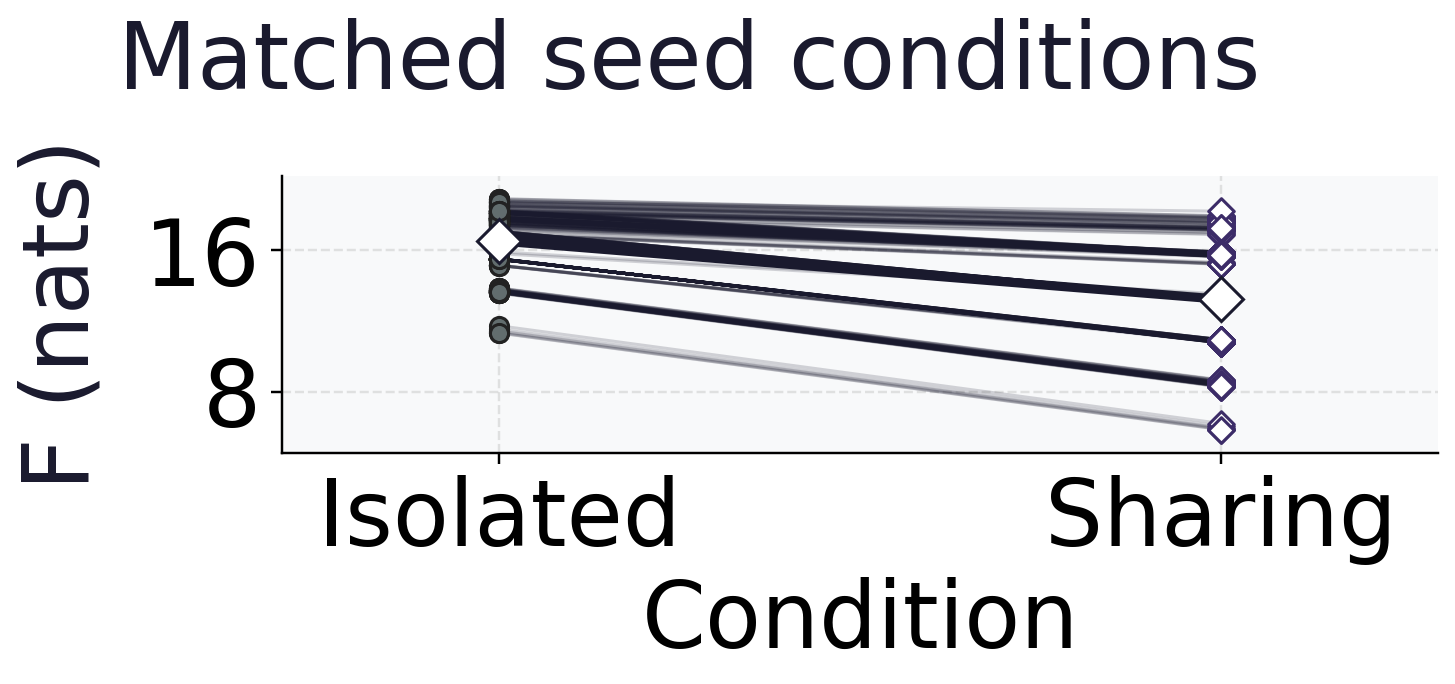
\includegraphics[keepaspectratio,width=0.98\linewidth,height=0.8\textheight,alt={Every seed connects its isolated and communicating colony mean; dark line with open diamonds marks condition means.}]{../figures/free_energy_comparison.slide-paired-seeds.png}
\refstepcounter{figure}\label{fig:free-energy-slide-panel-1}
\end{figure}
\end{frame}

\begin{frame}{Belief sharing lowers free\ldots{} (part 12)}
\begin{figure}
\centering
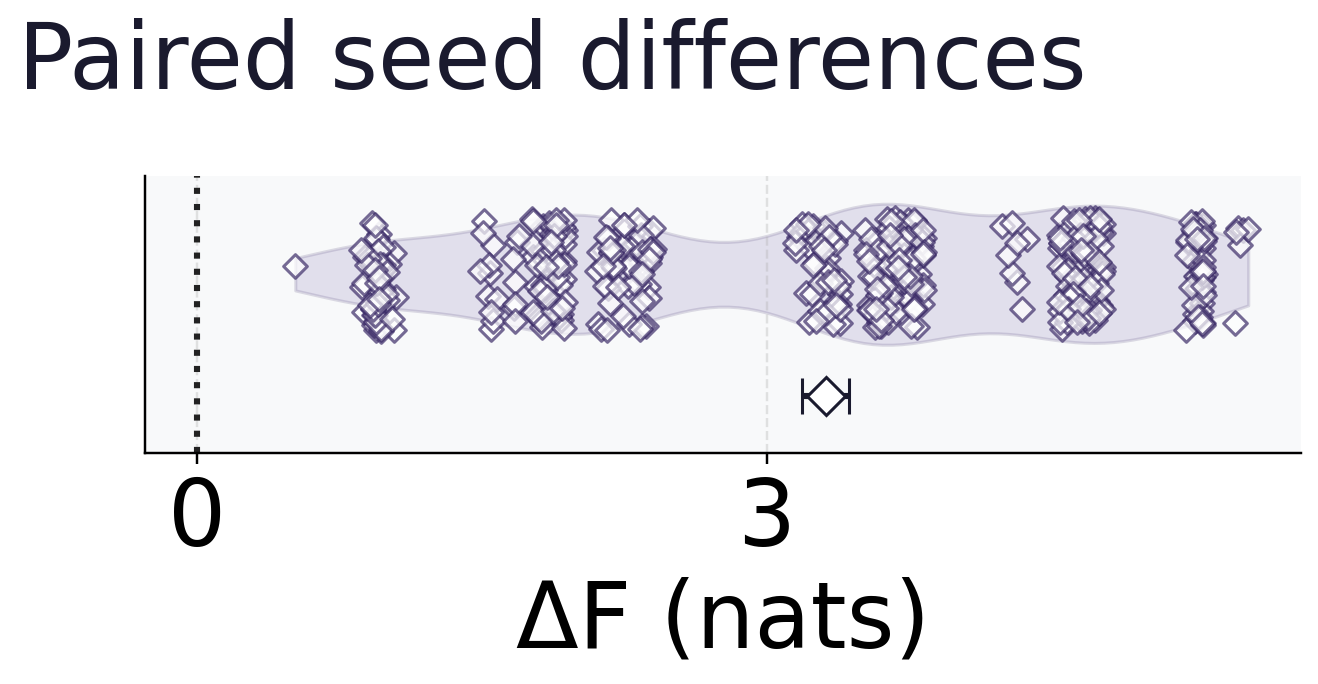
\includegraphics[keepaspectratio,width=0.98\linewidth,height=0.8\textheight,alt={All paired seed differences with jitter and descriptive violin, zero reference, and paired mean with the available report interval.}]{../figures/free_energy_comparison.slide-seed-differences.png}
\refstepcounter{figure}\label{fig:free-energy-slide-panel-2}
\end{figure}
\end{frame}

\begin{frame}{Belief sharing lowers free\ldots{} (part 13)}
\begin{figure}
\centering
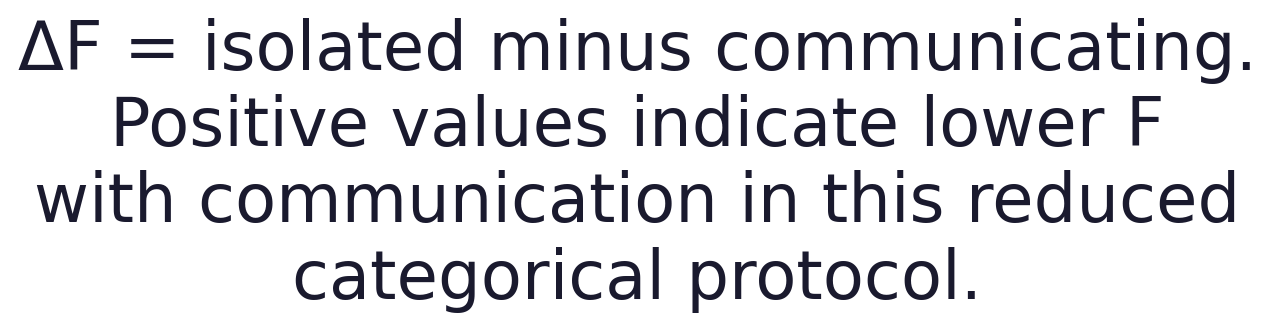
\includegraphics[keepaspectratio,width=0.98\linewidth,height=0.8\textheight,alt={ΔF = isolated minus communicating. Positive values indicate lower F with communication in this reduced categorical protocol.}]{../figures/free_energy_comparison.slide-direction.png}
\refstepcounter{figure}\label{fig:free-energy-slide-panel-3}
\end{figure}
\end{frame}

\begin{frame}{Belief sharing lowers free\ldots{} (part 14)}
\begin{figure}
\centering
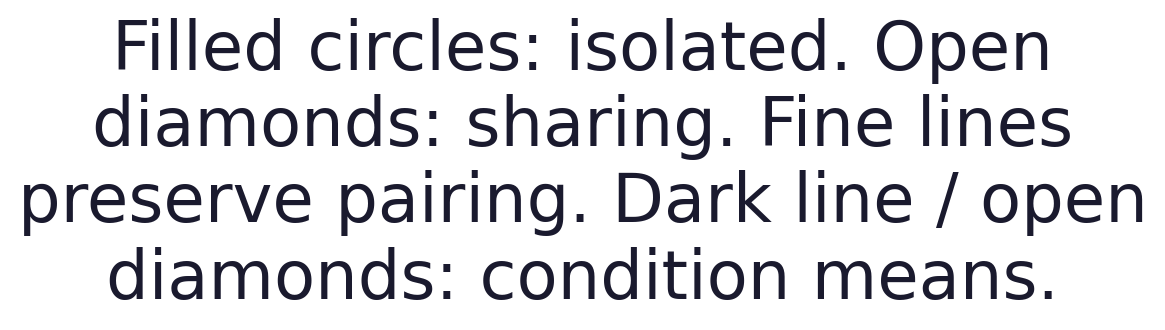
\includegraphics[keepaspectratio,width=0.98\linewidth,height=0.8\textheight,alt={Filled circles: isolated. Open diamonds: sharing. Fine lines preserve pairing. Dark line / open diamonds: condition means.}]{../figures/free_energy_comparison.slide-pair-key.png}
\refstepcounter{figure}\label{fig:free-energy-slide-panel-4}
\end{figure}
\end{frame}

\begin{frame}{Belief sharing lowers free\ldots{} (part 15)}
\begin{figure}
\centering
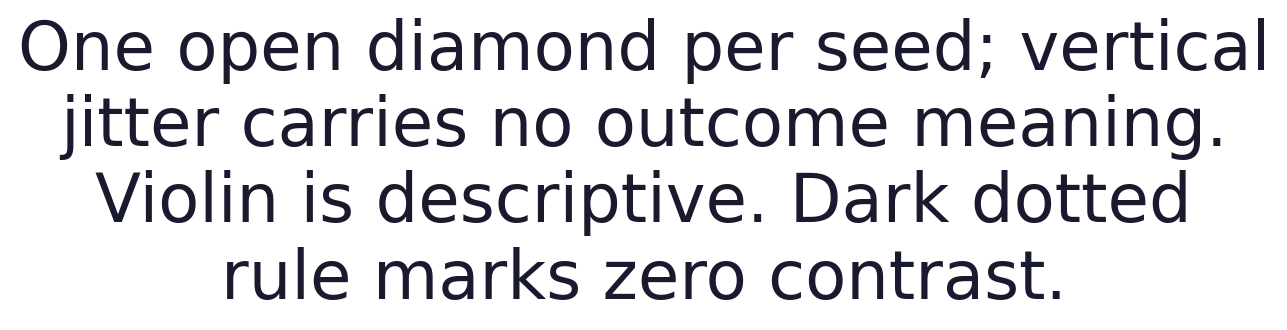
\includegraphics[keepaspectratio,width=0.98\linewidth,height=0.8\textheight,alt={One open diamond per seed; vertical jitter carries no outcome meaning. Violin is descriptive. Dark dotted rule marks zero contrast.}]{../figures/free_energy_comparison.slide-difference-key.png}
\refstepcounter{figure}\label{fig:free-energy-slide-panel-5}
\end{figure}
\end{frame}

\begin{frame}{Belief sharing lowers free\ldots{} (part 16)}
\begin{figure}
\centering

\includegraphics[keepaspectratio,width=0.98\linewidth,height=0.8\textheight,alt={Paired mean ΔF: +3.311 nats. Independent unit: configured seed; n = 480.}]{../figures/free_energy_comparison.slide-mean.png}
\refstepcounter{figure}\label{fig:free-energy-slide-panel-6}
\end{figure}
\end{frame}

\begin{frame}{Belief sharing lowers free\ldots{} (part 17)}
\begin{figure}
\centering
\includegraphics[keepaspectratio,width=0.98\linewidth,height=0.8\textheight,alt={Report-owned 95\% interval: {[}3.186, 3.433{]} nats.}]{../figures/free_energy_comparison.slide-interval.png}
\refstepcounter{figure}\label{fig:free-energy-slide-panel-7}
\end{figure}
\end{frame}

\begin{frame}{Belief sharing lowers free\ldots{} (part 18)}
\begin{figure}
\centering
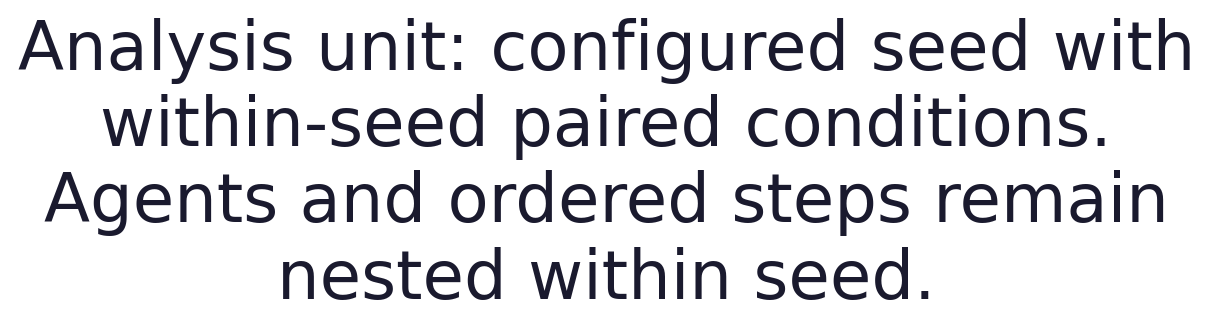
\includegraphics[keepaspectratio,width=0.98\linewidth,height=0.8\textheight,alt={Analysis unit: configured seed with within-seed paired conditions. Agents and ordered steps remain nested within seed.}]{../figures/free_energy_comparison.slide-unit.png}
\refstepcounter{figure}\label{fig:free-energy-slide-panel-8}
\end{figure}
\end{frame}

\begin{frame}{Belief sharing lowers free\ldots{} (part 19)}
\begin{figure}
\centering
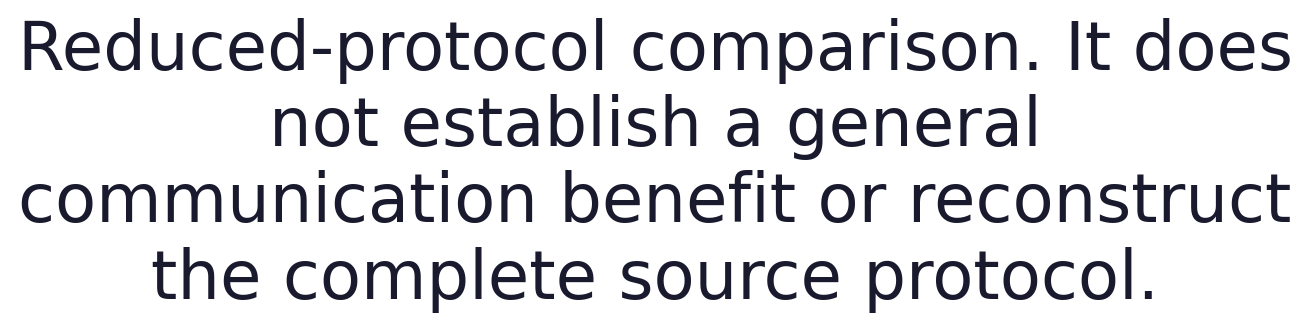
\includegraphics[keepaspectratio,width=0.98\linewidth,height=0.8\textheight,alt={Reduced-protocol comparison. It does not establish a general communication benefit or reconstruct the complete source protocol.}]{../figures/free_energy_comparison.slide-scope.png}
\refstepcounter{figure}\label{fig:free-energy-slide-panel-9}
\end{figure}
\end{frame}

\begin{frame}{Belief sharing lowers free\ldots{} (part 20)}
fig.~9 reports the headline gap;
fig.~10 shows the per-agent mechanism behind it.
\end{frame}

\begin{frame}{Belief sharing lowers free\ldots{} (part 21)}
\begin{figure}
\centering
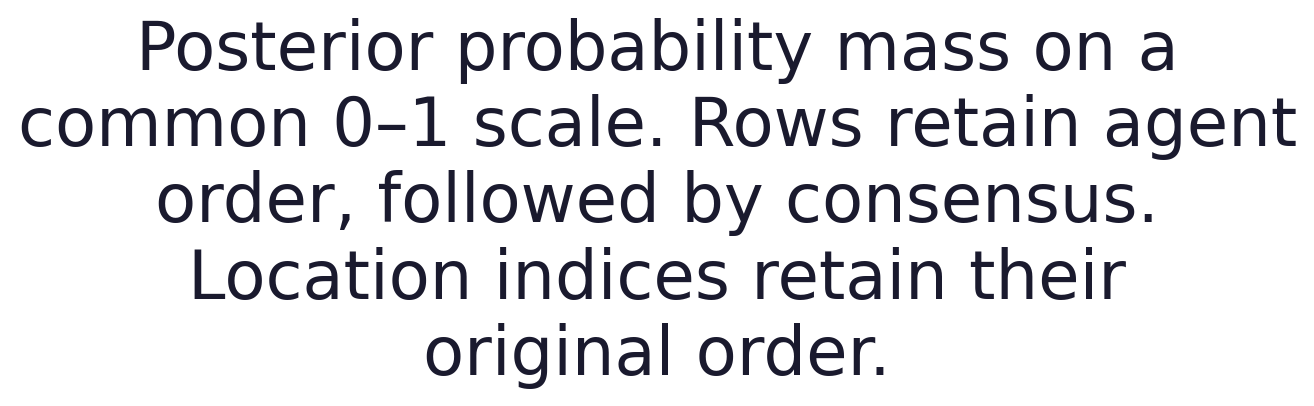
\includegraphics[keepaspectratio,width=0.98\linewidth,height=0.8\textheight,alt={Posterior probability mass on a common 0--1 scale. Rows retain agent order, followed by consensus. Location indices retain their original order.}]{../figures/belief_heatmap.slide-key.png}
\refstepcounter{figure}\label{fig:belief-heatmap-slide-panel-1}
\end{figure}
\end{frame}

\begin{frame}{Belief sharing lowers free\ldots{} (part 22)}
\begin{figure}
\centering
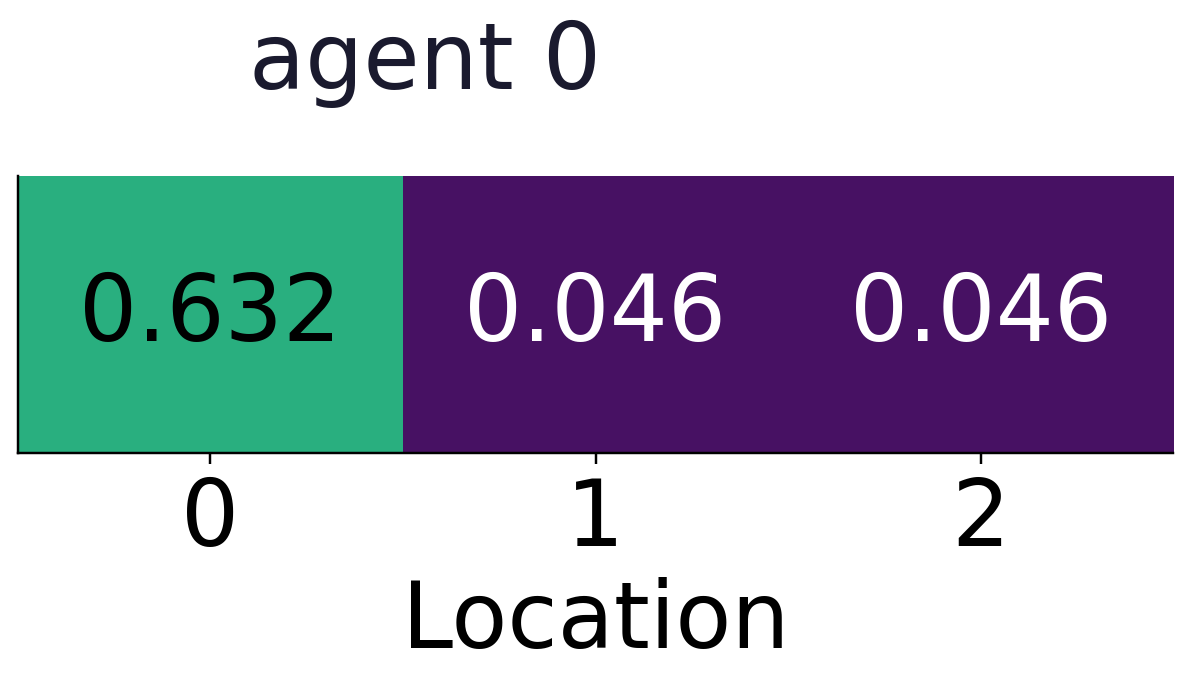
\includegraphics[keepaspectratio,width=0.98\linewidth,height=0.8\textheight,alt={agent 0, locations 0 through 2; every probability printed on the common 0--1 scale.}]{../figures/belief_heatmap.slide-row-0-cells-0-2.png}
\refstepcounter{figure}\label{fig:belief-heatmap-slide-panel-2}
\end{figure}
\end{frame}

\begin{frame}{Belief sharing lowers free\ldots{} (part 23)}
\begin{figure}
\centering
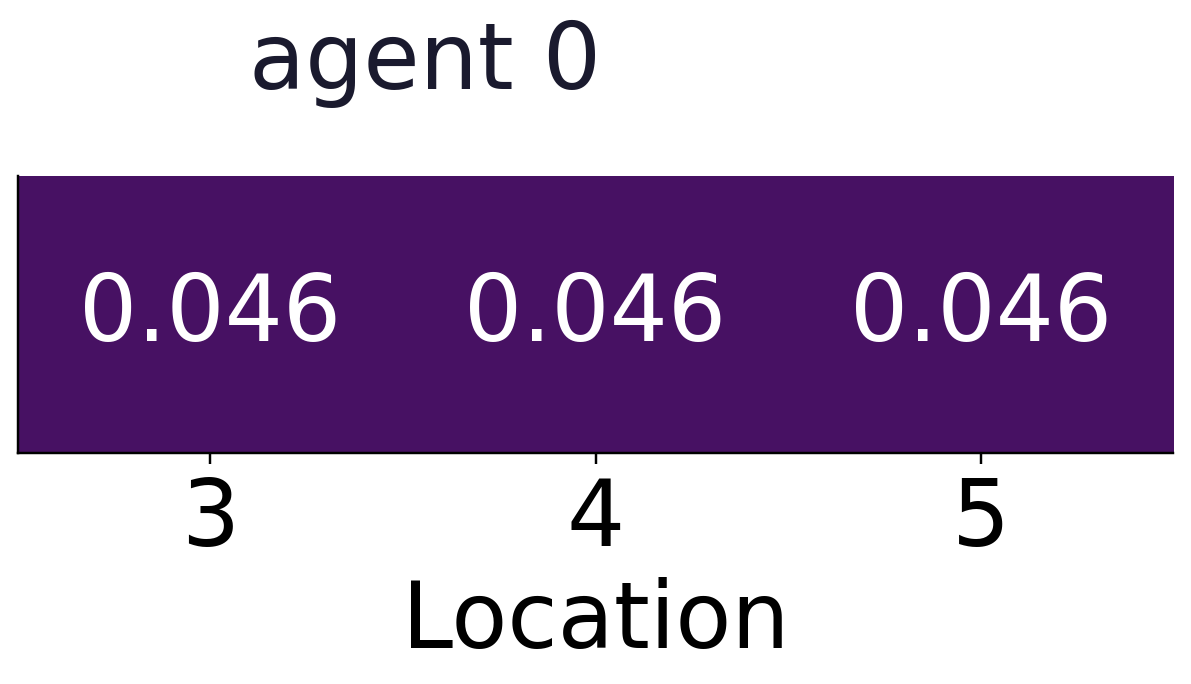
\includegraphics[keepaspectratio,width=0.98\linewidth,height=0.8\textheight,alt={agent 0, locations 3 through 5; every probability printed on the common 0--1 scale.}]{../figures/belief_heatmap.slide-row-0-cells-3-5.png}
\refstepcounter{figure}\label{fig:belief-heatmap-slide-panel-3}
\end{figure}
\end{frame}

\begin{frame}{Belief sharing lowers free\ldots{} (part 24)}
\begin{figure}
\centering
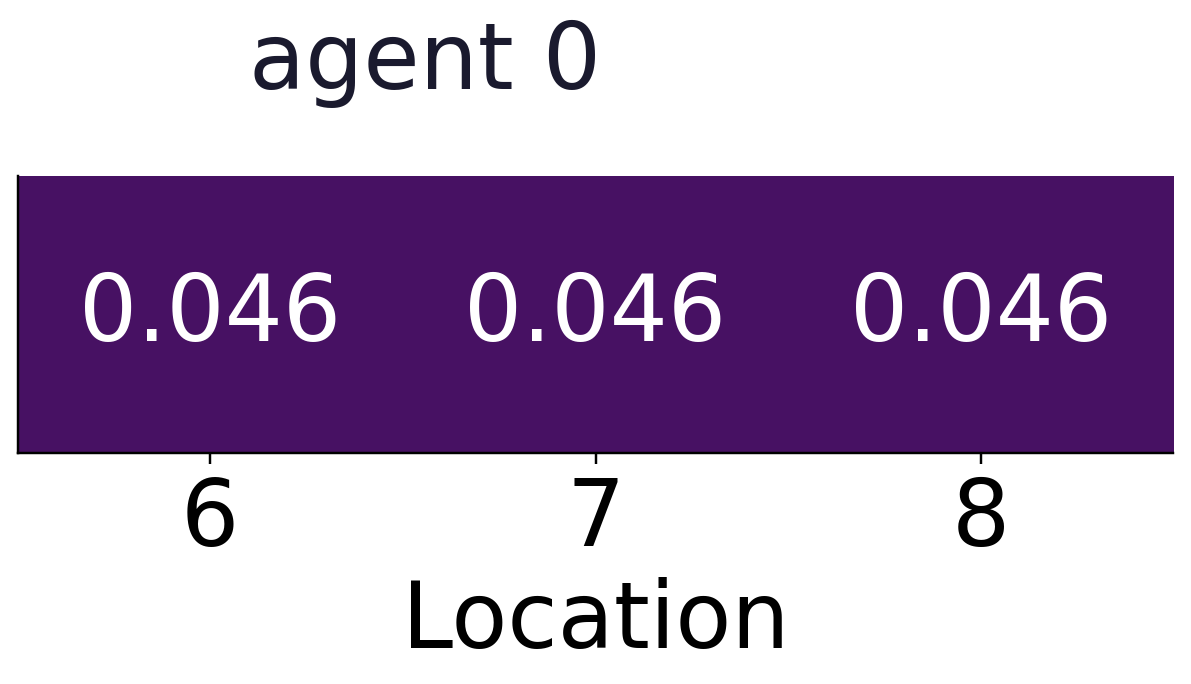
\includegraphics[keepaspectratio,width=0.98\linewidth,height=0.8\textheight,alt={agent 0, locations 6 through 8; every probability printed on the common 0--1 scale.}]{../figures/belief_heatmap.slide-row-0-cells-6-8.png}
\refstepcounter{figure}\label{fig:belief-heatmap-slide-panel-4}
\end{figure}
\end{frame}

\begin{frame}{Belief sharing lowers free\ldots{} (part 25)}
\begin{figure}
\centering
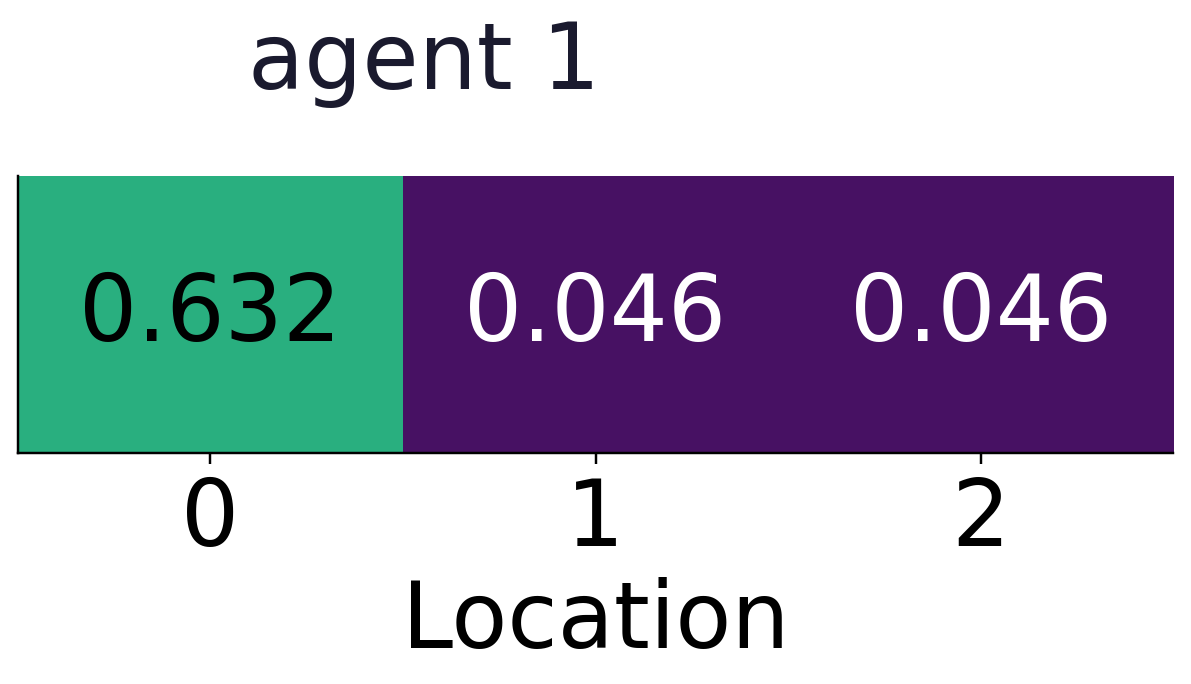
\includegraphics[keepaspectratio,width=0.98\linewidth,height=0.8\textheight,alt={agent 1, locations 0 through 2; every probability printed on the common 0--1 scale.}]{../figures/belief_heatmap.slide-row-1-cells-0-2.png}
\refstepcounter{figure}\label{fig:belief-heatmap-slide-panel-5}
\end{figure}
\end{frame}

\begin{frame}{Belief sharing lowers free\ldots{} (part 26)}
\begin{figure}
\centering
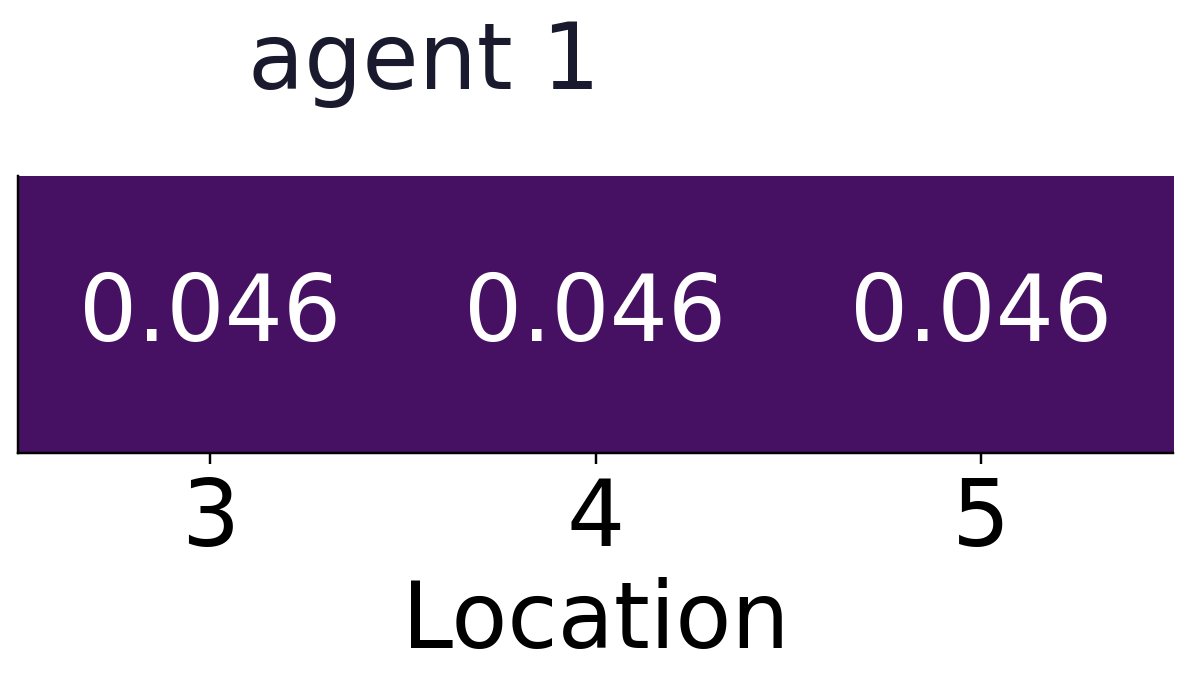
\includegraphics[keepaspectratio,width=0.98\linewidth,height=0.8\textheight,alt={agent 1, locations 3 through 5; every probability printed on the common 0--1 scale.}]{../figures/belief_heatmap.slide-row-1-cells-3-5.png}
\refstepcounter{figure}\label{fig:belief-heatmap-slide-panel-6}
\end{figure}
\end{frame}

\begin{frame}{Belief sharing lowers free\ldots{} (part 27)}
\begin{figure}
\centering
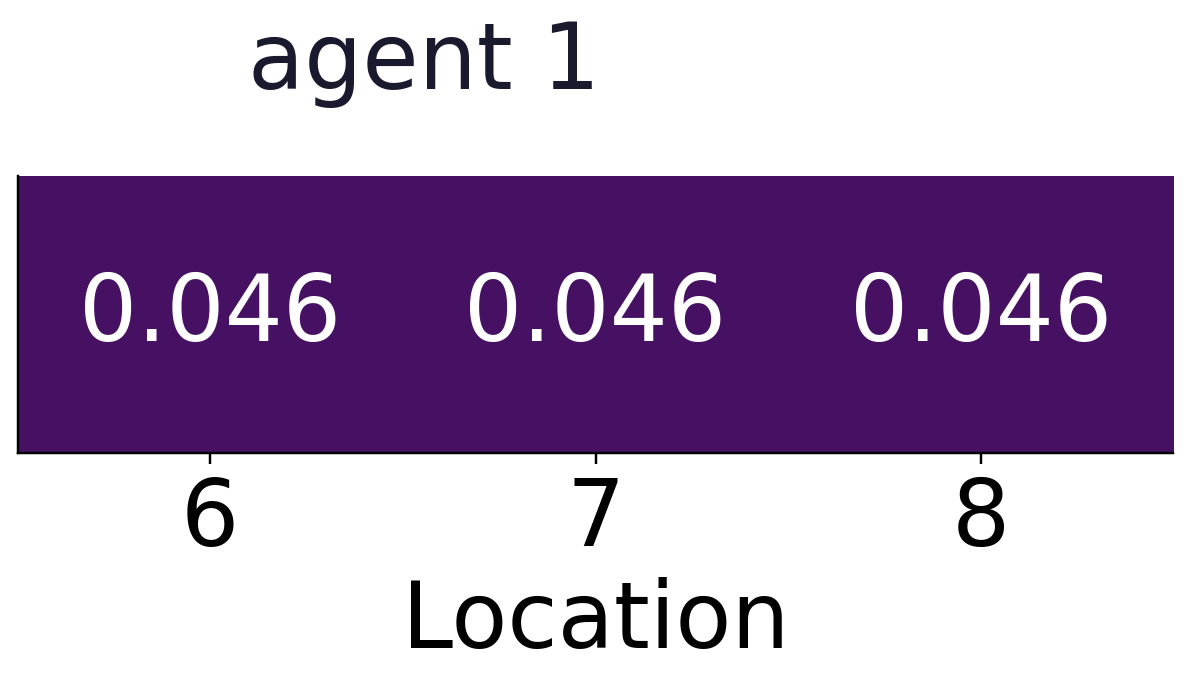
\includegraphics[keepaspectratio,width=0.98\linewidth,height=0.8\textheight,alt={agent 1, locations 6 through 8; every probability printed on the common 0--1 scale.}]{../figures/belief_heatmap.slide-row-1-cells-6-8.png}
\refstepcounter{figure}\label{fig:belief-heatmap-slide-panel-7}
\end{figure}
\end{frame}

\begin{frame}{Belief sharing lowers free\ldots{} (part 28)}
\begin{figure}
\centering
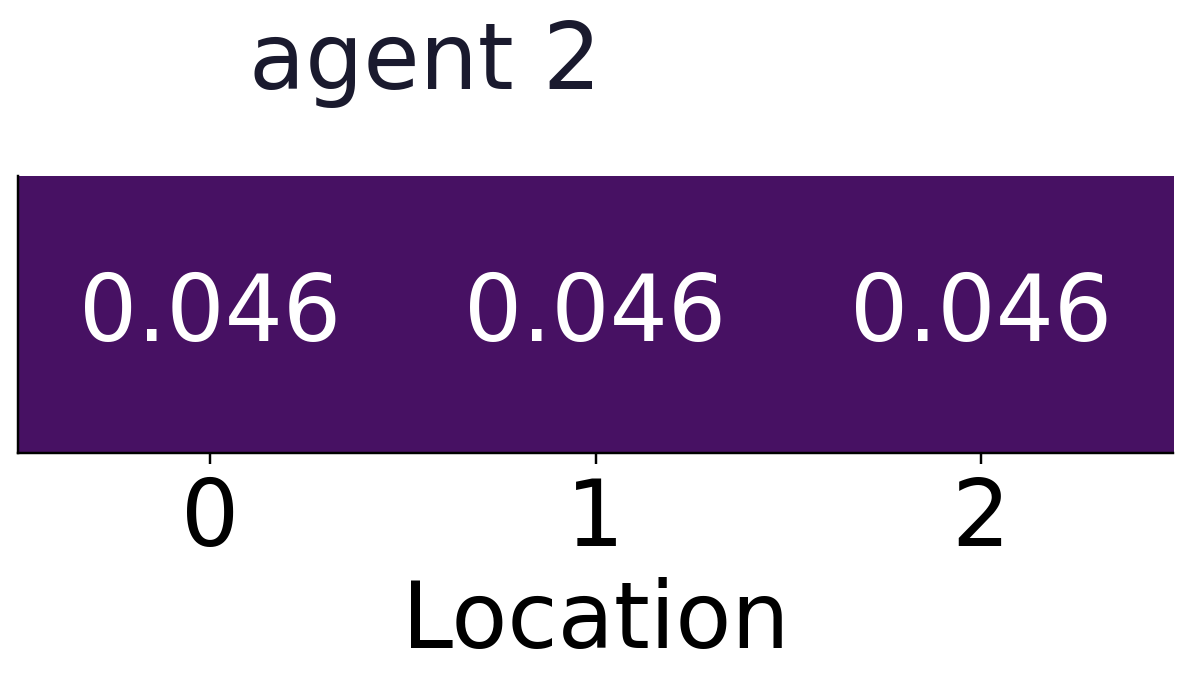
\includegraphics[keepaspectratio,width=0.98\linewidth,height=0.8\textheight,alt={agent 2, locations 0 through 2; every probability printed on the common 0--1 scale.}]{../figures/belief_heatmap.slide-row-2-cells-0-2.png}
\refstepcounter{figure}\label{fig:belief-heatmap-slide-panel-8}
\end{figure}
\end{frame}

\begin{frame}{Belief sharing lowers free\ldots{} (part 29)}
\begin{figure}
\centering
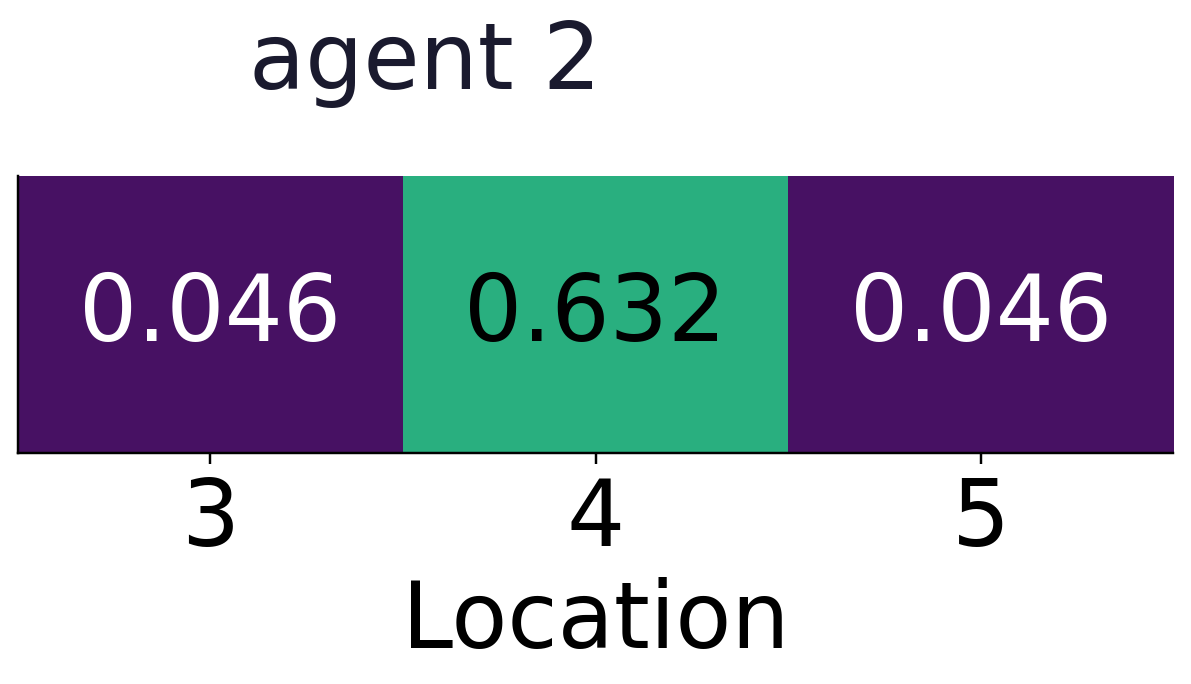
\includegraphics[keepaspectratio,width=0.98\linewidth,height=0.8\textheight,alt={agent 2, locations 3 through 5; every probability printed on the common 0--1 scale.}]{../figures/belief_heatmap.slide-row-2-cells-3-5.png}
\refstepcounter{figure}\label{fig:belief-heatmap-slide-panel-9}
\end{figure}
\end{frame}

\begin{frame}{Belief sharing lowers free\ldots{} (part 30)}
\begin{figure}
\centering
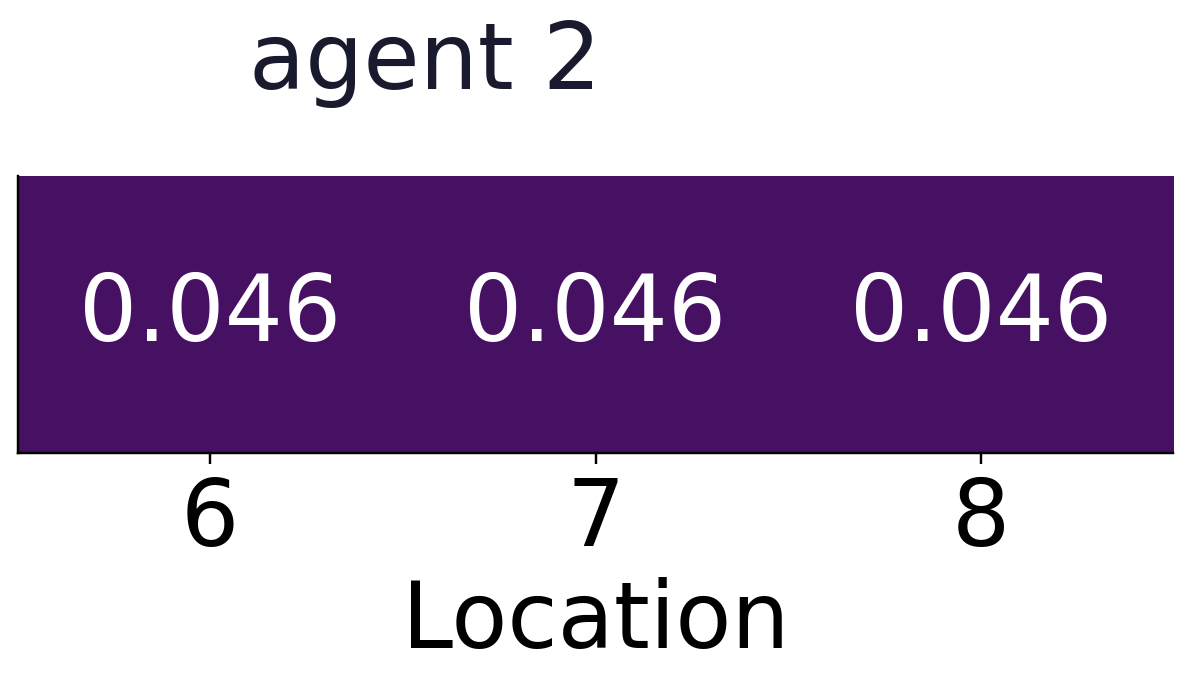
\includegraphics[keepaspectratio,width=0.98\linewidth,height=0.8\textheight,alt={agent 2, locations 6 through 8; every probability printed on the common 0--1 scale.}]{../figures/belief_heatmap.slide-row-2-cells-6-8.png}
\refstepcounter{figure}\label{fig:belief-heatmap-slide-panel-10}
\end{figure}
\end{frame}

\begin{frame}{Belief sharing lowers free\ldots{} (part 31)}
\begin{figure}
\centering
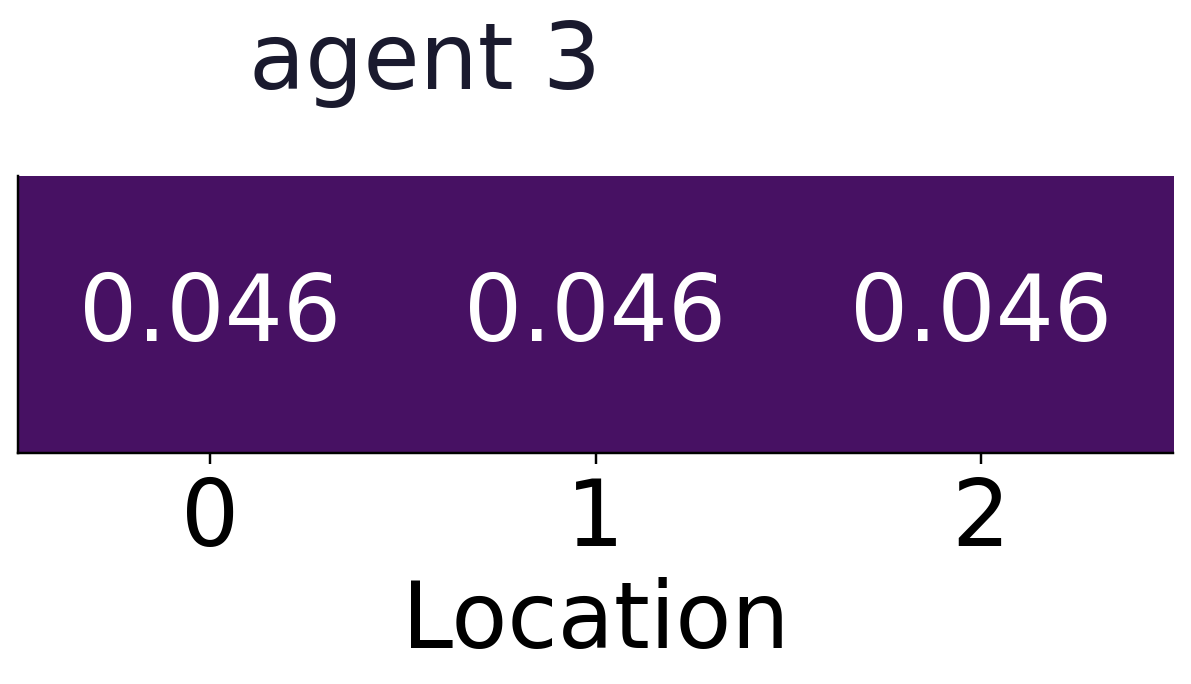
\includegraphics[keepaspectratio,width=0.98\linewidth,height=0.8\textheight,alt={agent 3, locations 0 through 2; every probability printed on the common 0--1 scale.}]{../figures/belief_heatmap.slide-row-3-cells-0-2.png}
\refstepcounter{figure}\label{fig:belief-heatmap-slide-panel-11}
\end{figure}
\end{frame}

\begin{frame}{Belief sharing lowers free\ldots{} (part 32)}
\begin{figure}
\centering
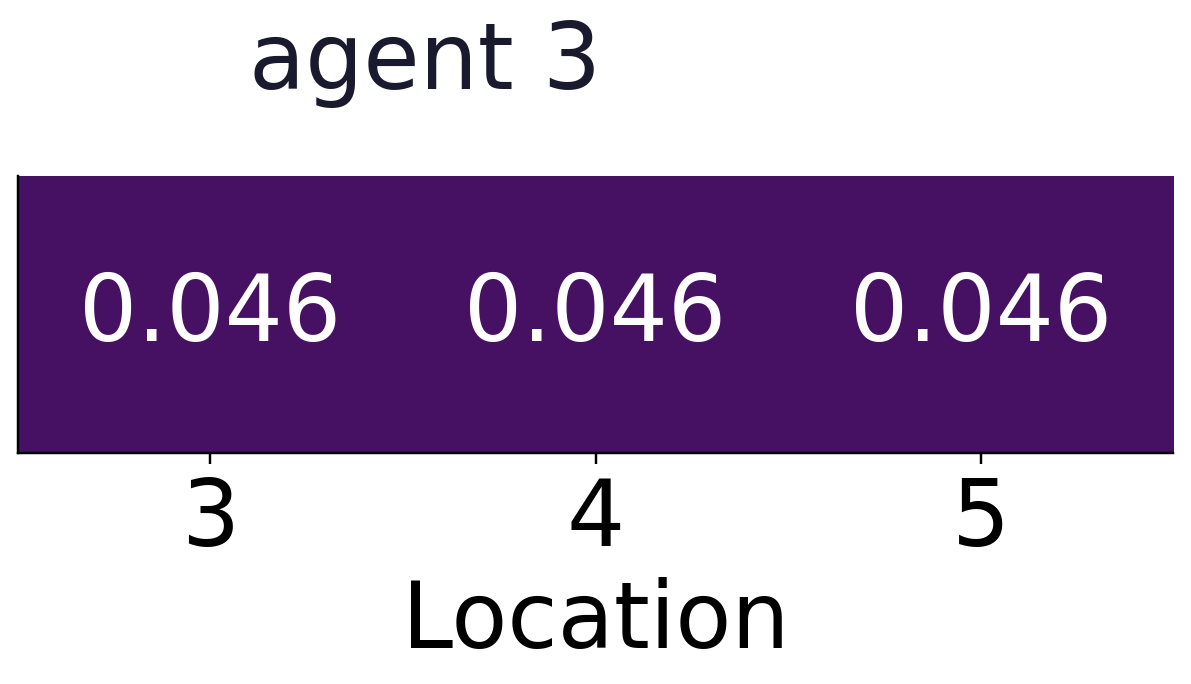
\includegraphics[keepaspectratio,width=0.98\linewidth,height=0.8\textheight,alt={agent 3, locations 3 through 5; every probability printed on the common 0--1 scale.}]{../figures/belief_heatmap.slide-row-3-cells-3-5.png}
\refstepcounter{figure}\label{fig:belief-heatmap-slide-panel-12}
\end{figure}
\end{frame}

\begin{frame}{Belief sharing lowers free\ldots{} (part 33)}
\begin{figure}
\centering
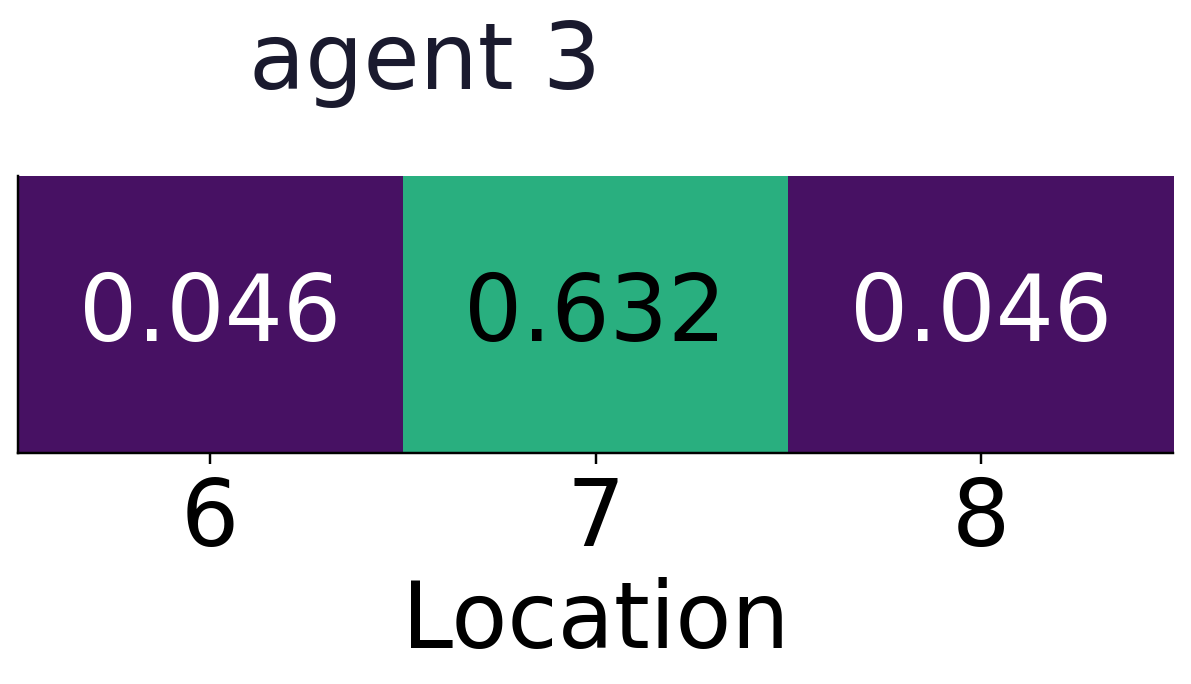
\includegraphics[keepaspectratio,width=0.98\linewidth,height=0.8\textheight,alt={agent 3, locations 6 through 8; every probability printed on the common 0--1 scale.}]{../figures/belief_heatmap.slide-row-3-cells-6-8.png}
\refstepcounter{figure}\label{fig:belief-heatmap-slide-panel-13}
\end{figure}
\end{frame}

\begin{frame}{Belief sharing lowers free\ldots{} (part 34)}
\begin{figure}
\centering
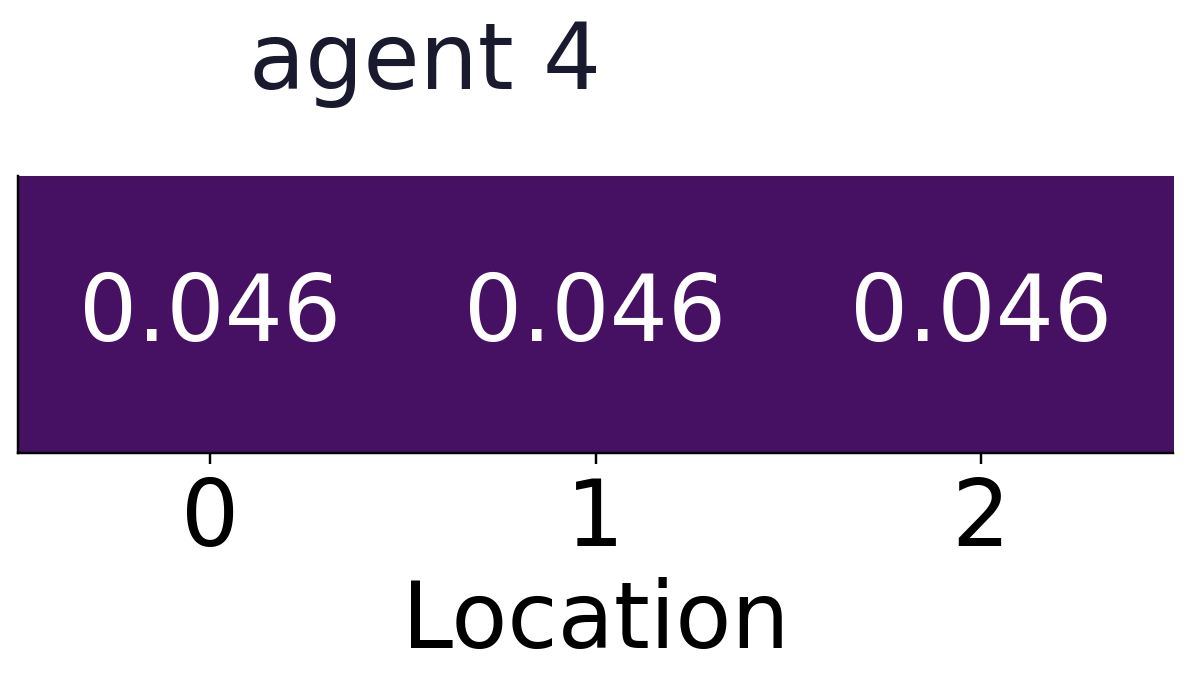
\includegraphics[keepaspectratio,width=0.98\linewidth,height=0.8\textheight,alt={agent 4, locations 0 through 2; every probability printed on the common 0--1 scale.}]{../figures/belief_heatmap.slide-row-4-cells-0-2.png}
\refstepcounter{figure}\label{fig:belief-heatmap-slide-panel-14}
\end{figure}
\end{frame}

\begin{frame}{Belief sharing lowers free\ldots{} (part 35)}
\begin{figure}
\centering
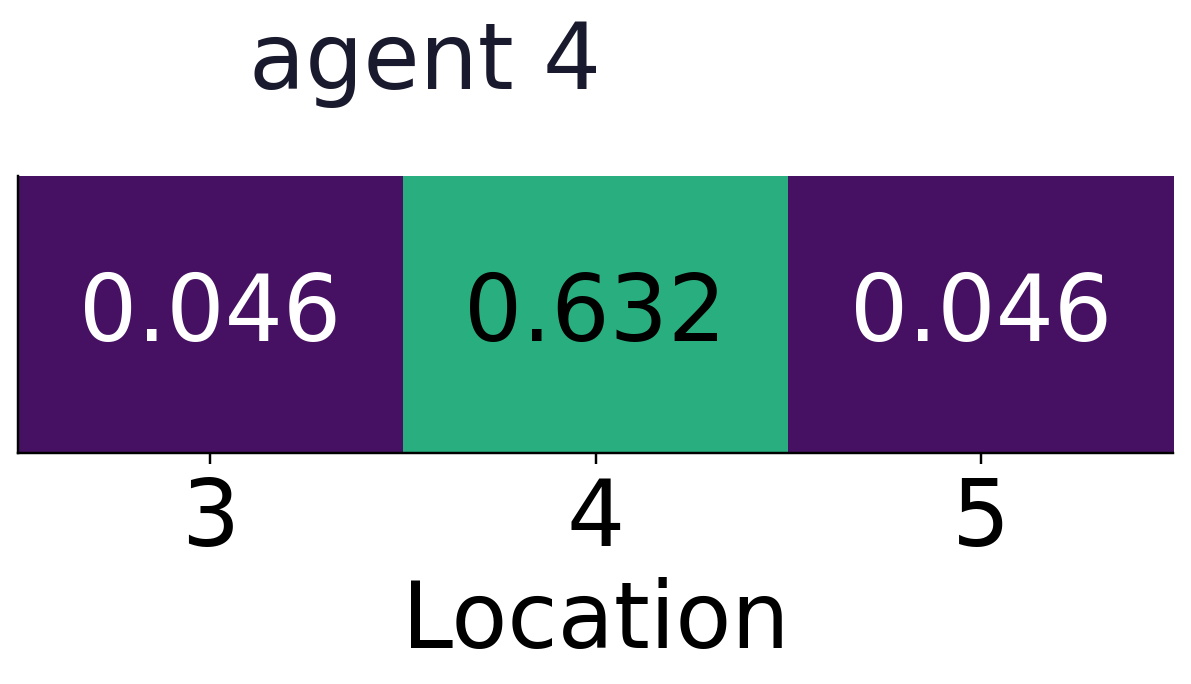
\includegraphics[keepaspectratio,width=0.98\linewidth,height=0.8\textheight,alt={agent 4, locations 3 through 5; every probability printed on the common 0--1 scale.}]{../figures/belief_heatmap.slide-row-4-cells-3-5.png}
\refstepcounter{figure}\label{fig:belief-heatmap-slide-panel-15}
\end{figure}
\end{frame}

\begin{frame}{Belief sharing lowers free\ldots{} (part 36)}
\begin{figure}
\centering
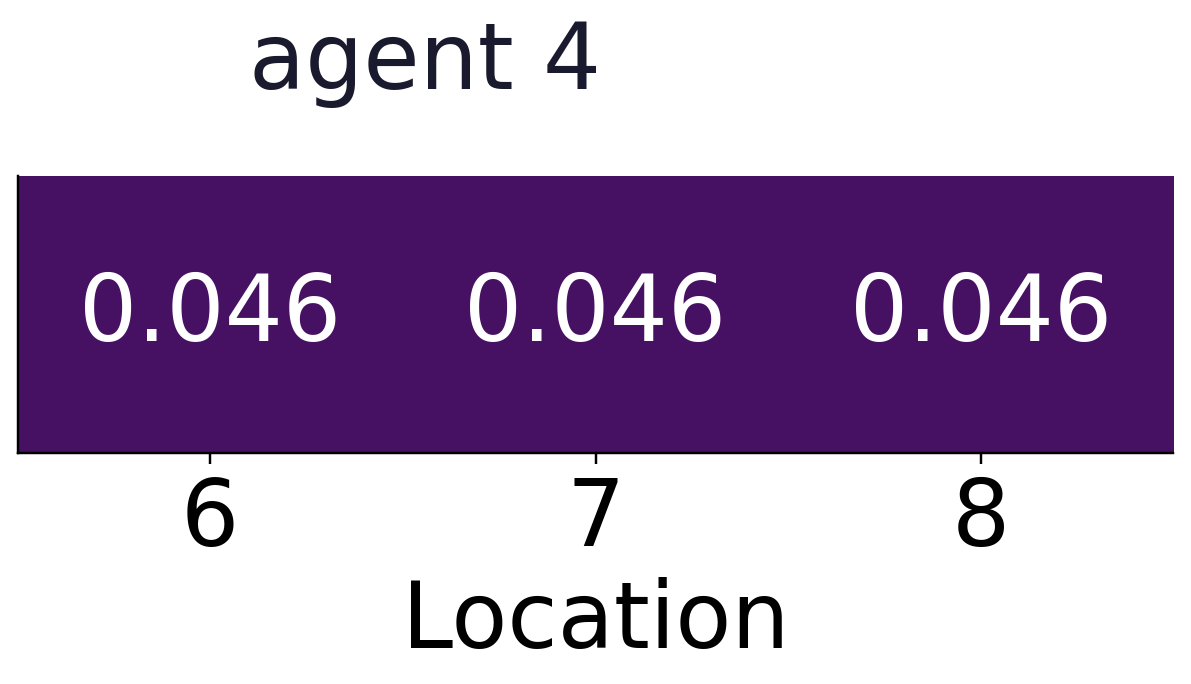
\includegraphics[keepaspectratio,width=0.98\linewidth,height=0.8\textheight,alt={agent 4, locations 6 through 8; every probability printed on the common 0--1 scale.}]{../figures/belief_heatmap.slide-row-4-cells-6-8.png}
\refstepcounter{figure}\label{fig:belief-heatmap-slide-panel-16}
\end{figure}
\end{frame}

\begin{frame}{Belief sharing lowers free\ldots{} (part 37)}
\begin{figure}
\centering
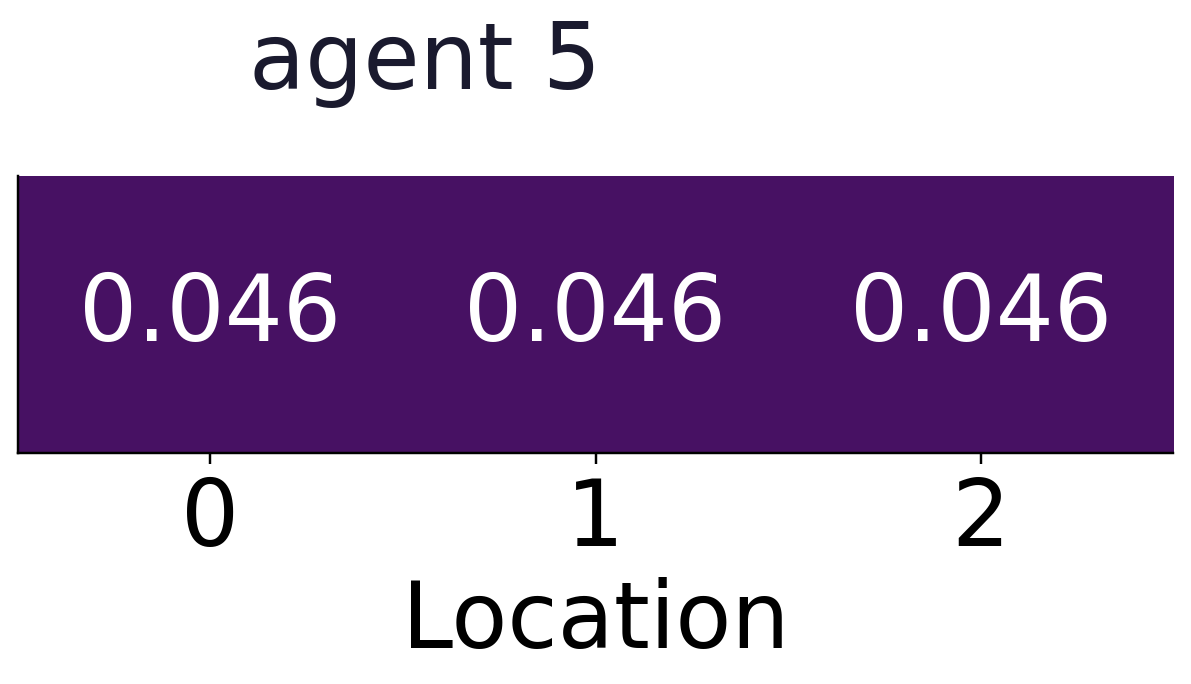
\includegraphics[keepaspectratio,width=0.98\linewidth,height=0.8\textheight,alt={agent 5, locations 0 through 2; every probability printed on the common 0--1 scale.}]{../figures/belief_heatmap.slide-row-5-cells-0-2.png}
\refstepcounter{figure}\label{fig:belief-heatmap-slide-panel-17}
\end{figure}
\end{frame}

\begin{frame}{Belief sharing lowers free\ldots{} (part 38)}
\begin{figure}
\centering
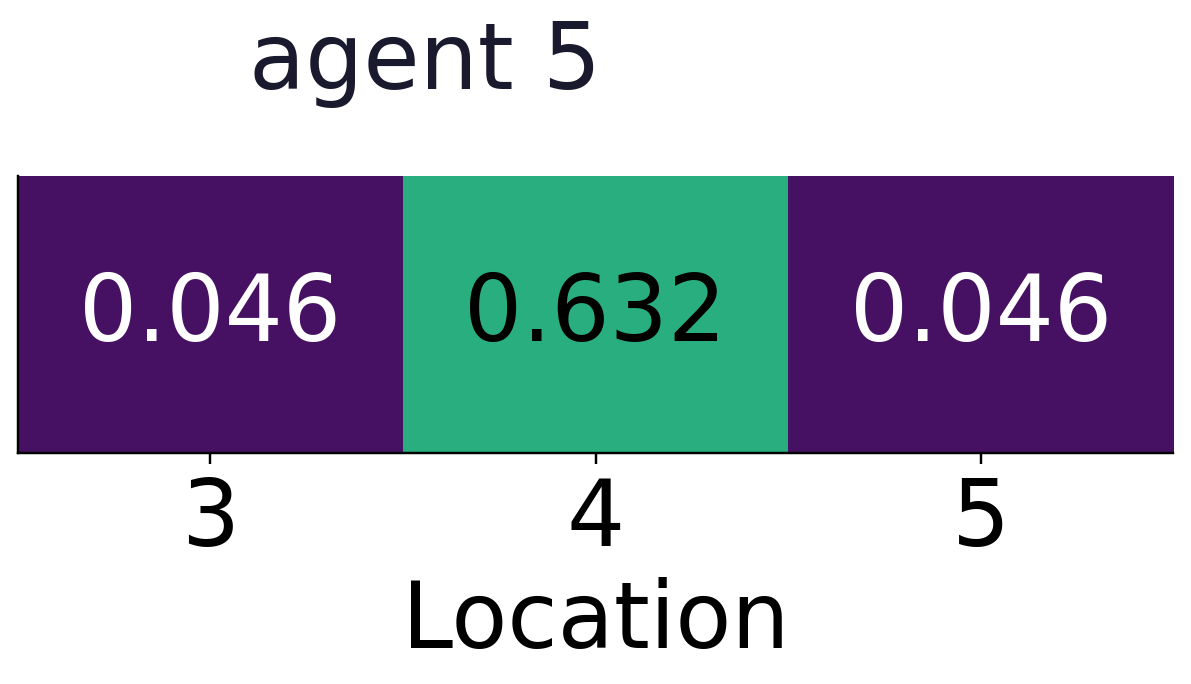
\includegraphics[keepaspectratio,width=0.98\linewidth,height=0.8\textheight,alt={agent 5, locations 3 through 5; every probability printed on the common 0--1 scale.}]{../figures/belief_heatmap.slide-row-5-cells-3-5.png}
\refstepcounter{figure}\label{fig:belief-heatmap-slide-panel-18}
\end{figure}
\end{frame}

\begin{frame}{Belief sharing lowers free\ldots{} (part 39)}
\begin{figure}
\centering
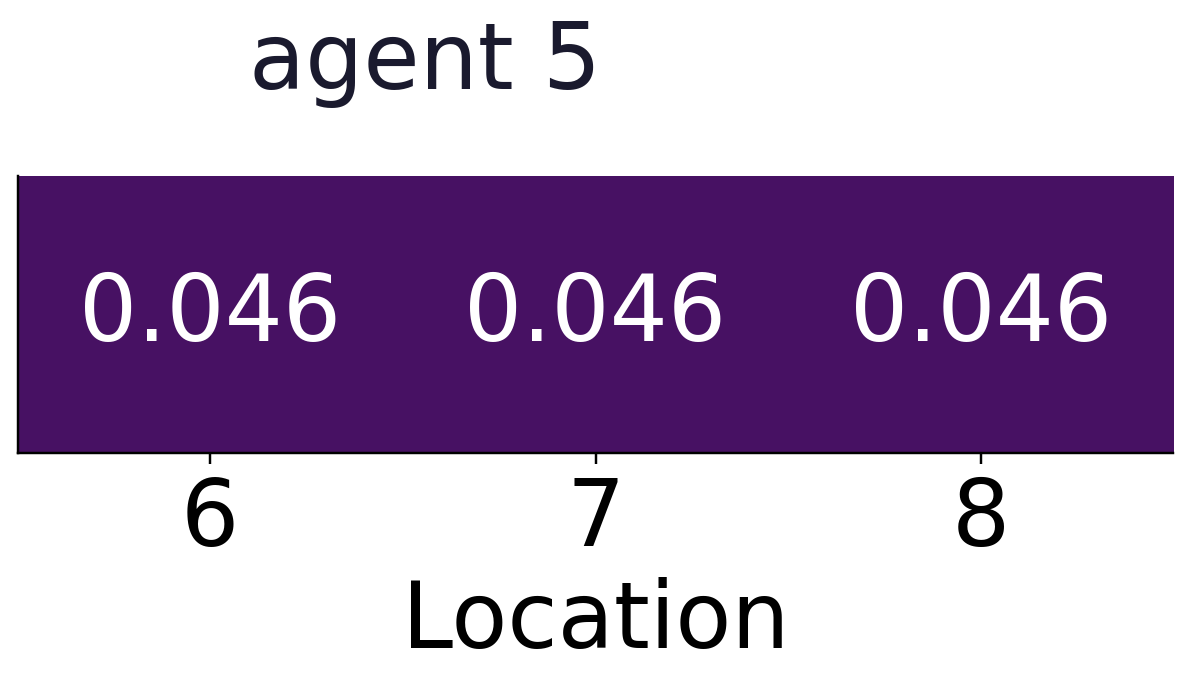
\includegraphics[keepaspectratio,width=0.98\linewidth,height=0.8\textheight,alt={agent 5, locations 6 through 8; every probability printed on the common 0--1 scale.}]{../figures/belief_heatmap.slide-row-5-cells-6-8.png}
\refstepcounter{figure}\label{fig:belief-heatmap-slide-panel-19}
\end{figure}
\end{frame}

\begin{frame}{Belief sharing lowers free\ldots{} (part 40)}
\begin{figure}
\centering
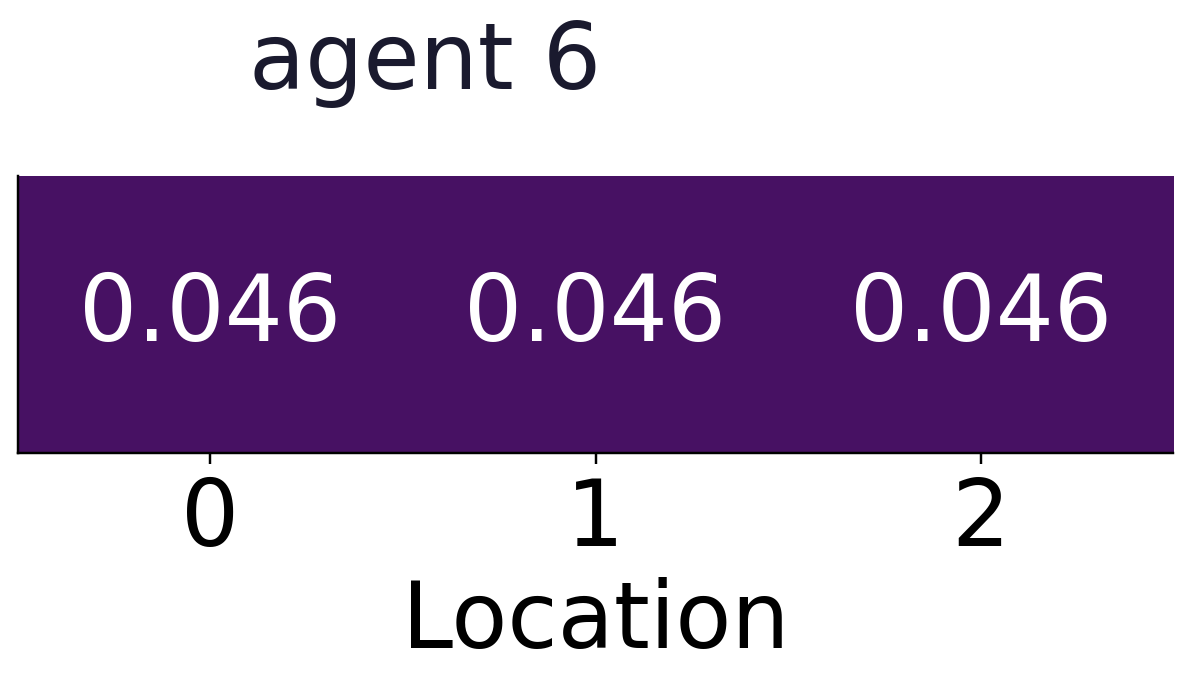
\includegraphics[keepaspectratio,width=0.98\linewidth,height=0.8\textheight,alt={agent 6, locations 0 through 2; every probability printed on the common 0--1 scale.}]{../figures/belief_heatmap.slide-row-6-cells-0-2.png}
\refstepcounter{figure}\label{fig:belief-heatmap-slide-panel-20}
\end{figure}
\end{frame}

\begin{frame}{Belief sharing lowers free\ldots{} (part 41)}
\begin{figure}
\centering
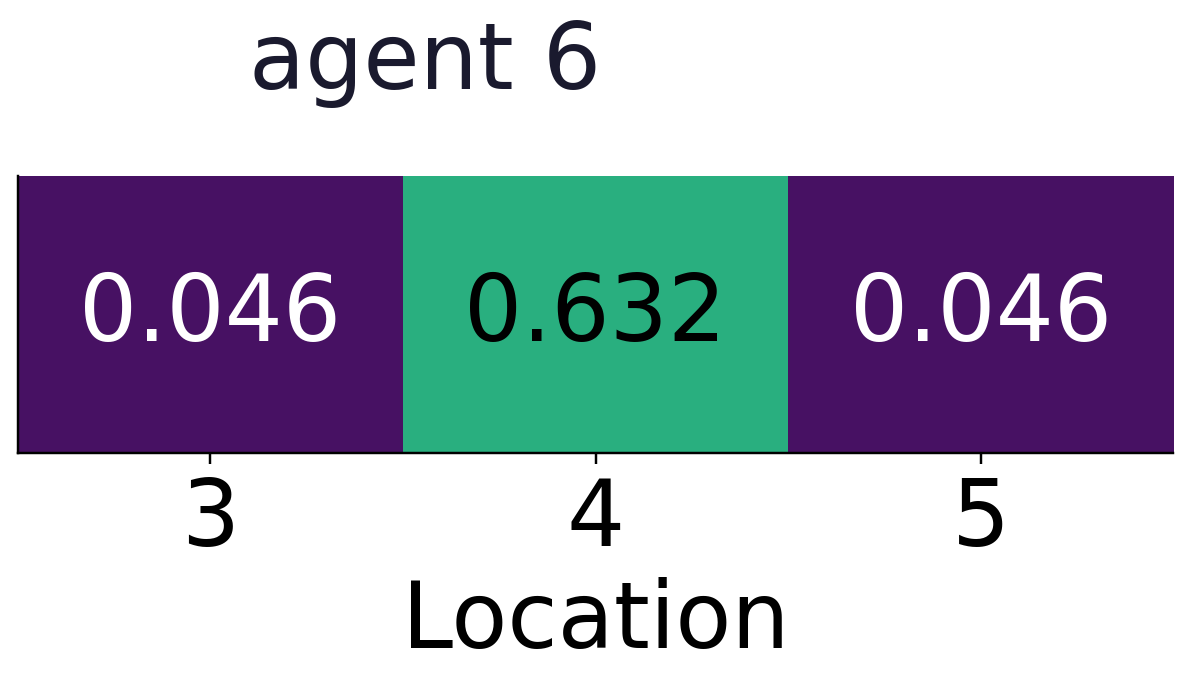
\includegraphics[keepaspectratio,width=0.98\linewidth,height=0.8\textheight,alt={agent 6, locations 3 through 5; every probability printed on the common 0--1 scale.}]{../figures/belief_heatmap.slide-row-6-cells-3-5.png}
\refstepcounter{figure}\label{fig:belief-heatmap-slide-panel-21}
\end{figure}
\end{frame}

\begin{frame}{Belief sharing lowers free\ldots{} (part 42)}
\begin{figure}
\centering
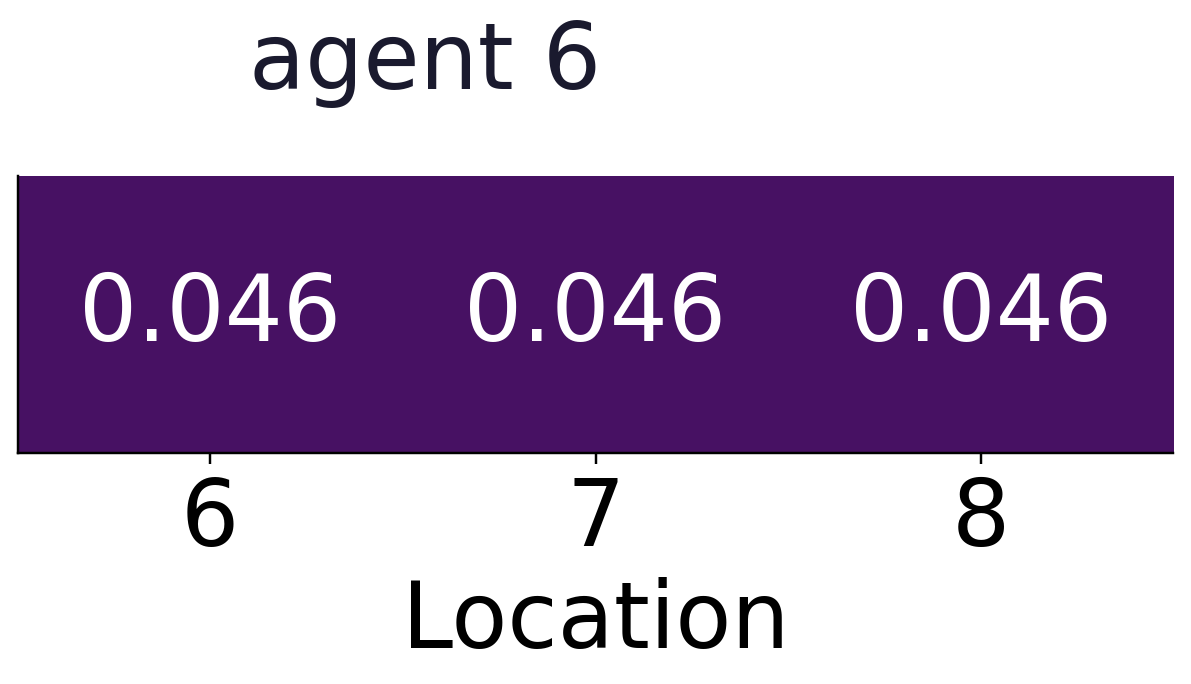
\includegraphics[keepaspectratio,width=0.98\linewidth,height=0.8\textheight,alt={agent 6, locations 6 through 8; every probability printed on the common 0--1 scale.}]{../figures/belief_heatmap.slide-row-6-cells-6-8.png}
\refstepcounter{figure}\label{fig:belief-heatmap-slide-panel-22}
\end{figure}
\end{frame}

\begin{frame}{Belief sharing lowers free\ldots{} (part 43)}
\begin{figure}
\centering
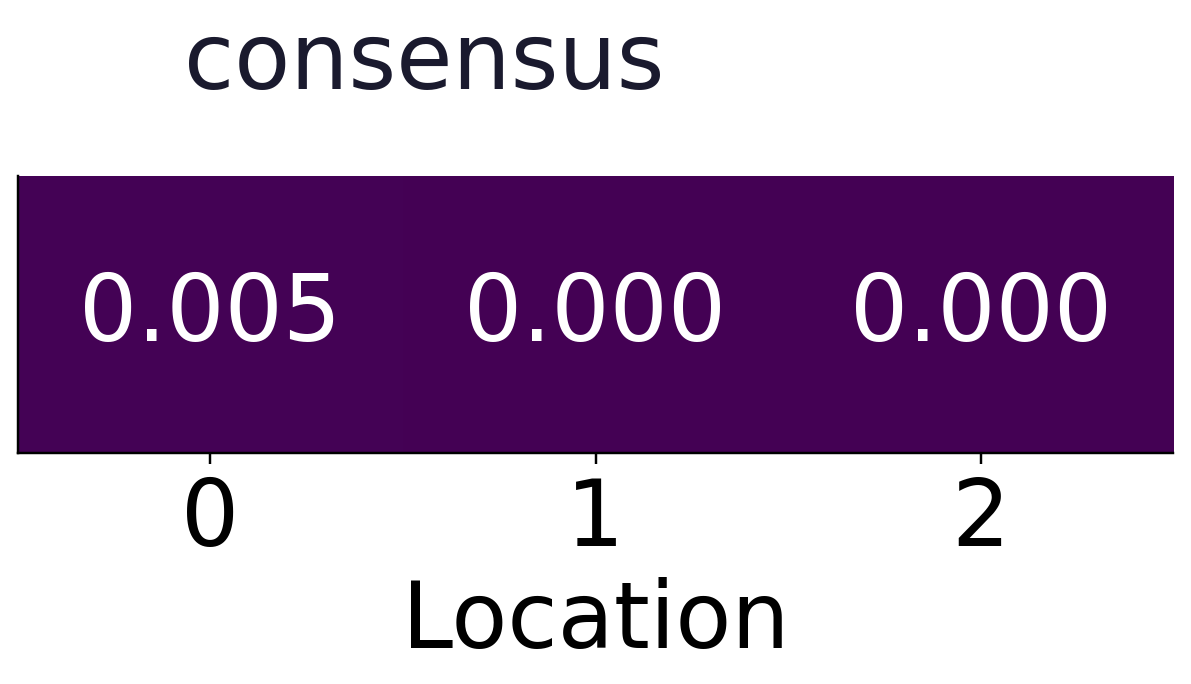
\includegraphics[keepaspectratio,width=0.98\linewidth,height=0.8\textheight,alt={consensus, locations 0 through 2; every probability printed on the common 0--1 scale.}]{../figures/belief_heatmap.slide-row-7-cells-0-2.png}
\refstepcounter{figure}\label{fig:belief-heatmap-slide-panel-23}
\end{figure}
\end{frame}

\begin{frame}{Belief sharing lowers free\ldots{} (part 44)}
\begin{figure}
\centering
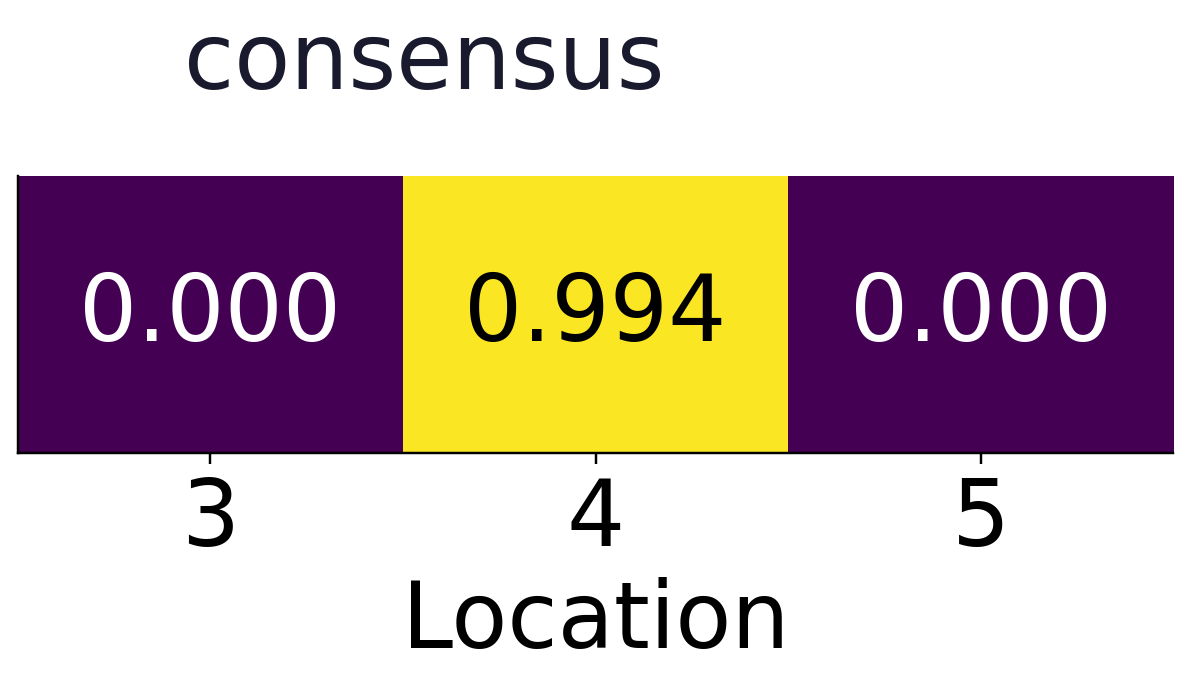
\includegraphics[keepaspectratio,width=0.98\linewidth,height=0.8\textheight,alt={consensus, locations 3 through 5; every probability printed on the common 0--1 scale.}]{../figures/belief_heatmap.slide-row-7-cells-3-5.png}
\refstepcounter{figure}\label{fig:belief-heatmap-slide-panel-24}
\end{figure}
\end{frame}

\begin{frame}{Belief sharing lowers free\ldots{} (part 45)}
\begin{figure}
\centering
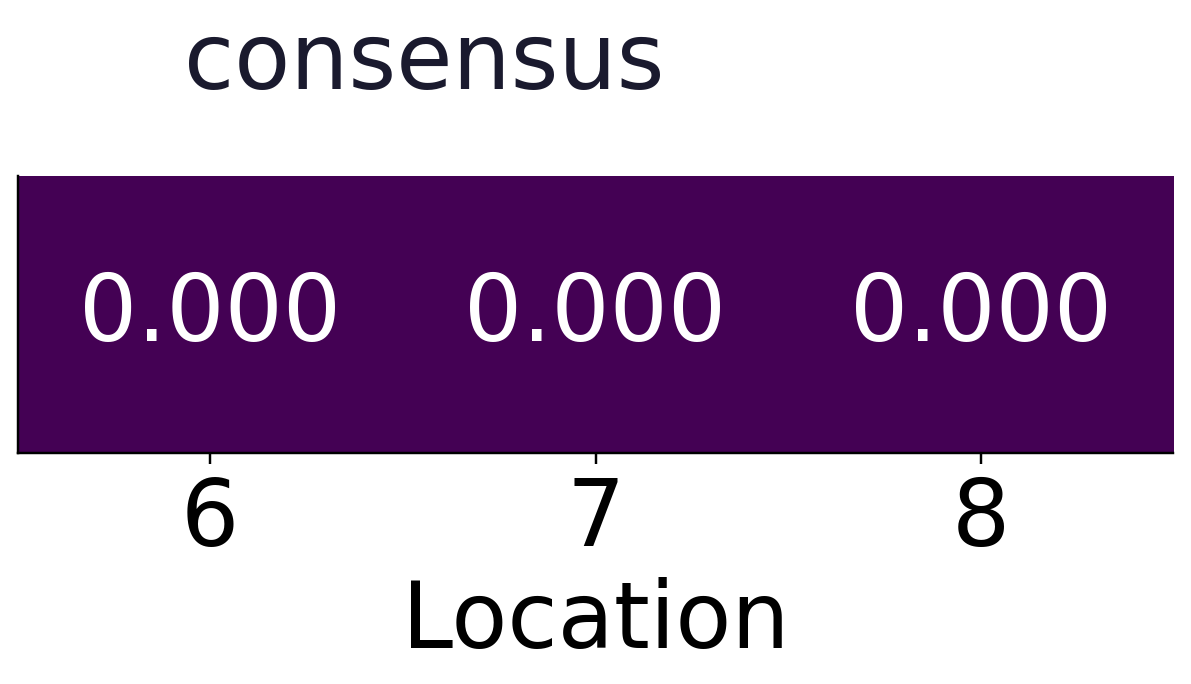
\includegraphics[keepaspectratio,width=0.98\linewidth,height=0.8\textheight,alt={consensus, locations 6 through 8; every probability printed on the common 0--1 scale.}]{../figures/belief_heatmap.slide-row-7-cells-6-8.png}
\refstepcounter{figure}\label{fig:belief-heatmap-slide-panel-25}
\end{figure}
\end{frame}

\begin{frame}{Belief sharing lowers free\ldots{} (part 46)}
\begin{figure}
\centering
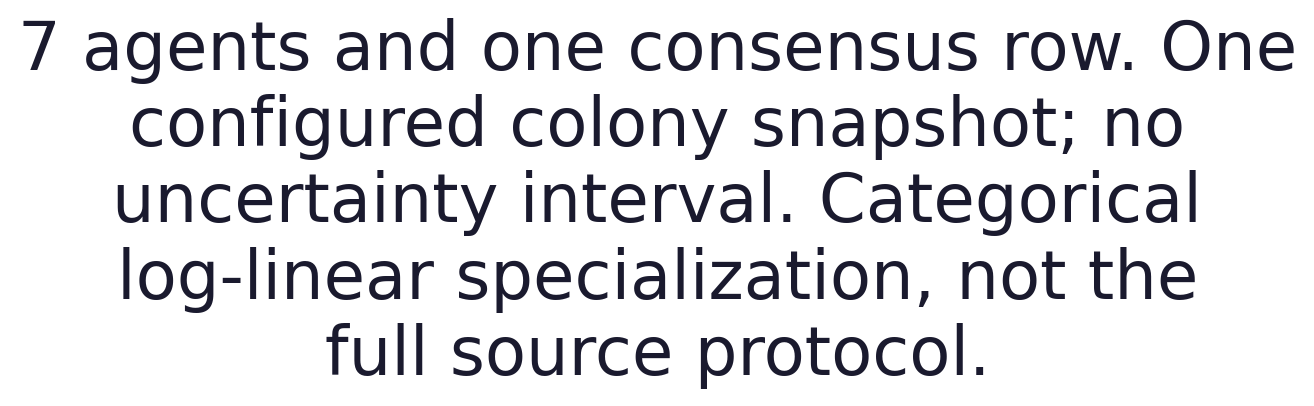
\includegraphics[keepaspectratio,width=0.98\linewidth,height=0.8\textheight,alt={7 agents and one consensus row. One configured colony snapshot; no uncertainty interval. Categorical log-linear specialization, not the full source protocol.}]{../figures/belief_heatmap.slide-scope.png}
\refstepcounter{figure}\label{fig:belief-heatmap-slide-panel-26}
\end{figure}
\end{frame}

\begin{frame}{Three robustness axes remain distinct in the results}
\protect\phantomsection\label{sec:robustness-axes-results}
The authoritative three-axis guarantee map is
sec.~3.3. The contaminated studies keep its
source-conditional client update, heuristic server reweighting,
\end{frame}

\begin{frame}[fragile]{Three robustness axes\ldots{} (part 2)}
and objective-backed variational server rule visually and inferentially
separate. In particular, no result below transfers the client's
bounded-influence theorem or the variational rule's raw-weight bound to
\texttt{robust\_aggregate}.
\end{frame}

\end{document}
